\chapter{Modelo Proposto}
\label{cap:sistema_proposto}

% Geladeiras inteligentes existentes
    % Funcionalidades

Este capítulo tem por objetivo detalhar o sistema proposto apresentando uma visão lógica e uma visão física promovendo, assim, um entendimento do como os diversos componentes interagem e se comportam.

\section{Introdução}

Geladeiras inteligentes têm sido lançadas por fabricantes como Samsung\textsuperscript{\textregistered} e LG\textsuperscript{\textregistered}, tendo estas muitas características em comum. Em relação ao modelo tradicional, essas geladeiras proporcionam uma maior interação com os usuários a partir de uma interface \textit{touch screen}, além do uso de câmeras no interior do equipamento.

A partir da interface é possível criar lembretes para os demais moradores da casa, ler notícias e ver a previsão do tempo. Além disso, é possível adicionar itens ao calendário e visualizar receitas. Por outro lado, conta-se com o auxílio de assistentes virtuais como a Alexa\textsuperscript{\textregistered}, da Amazon\textsuperscript{\textregistered}, e a Cortana\textsuperscript{\textregistered} da Microsoft\textsuperscript{\textregistered}, que possibilitam que ações sejam executadas a partir de comandos de voz como, por exemplo, compras de novos produtos. 

Apesar de as funcionalidades serem úteis e interessantes, geladeiras como estas não observam os hábitos e preferências por produtos de seus usuários. Como exemplo, tais eletrodomésticos não são capazes de inferir que um usuário seja vegetariano ou que tenha intolerância à lactose.

    
% Componentes do sistema (geladeira, aTTplicação, servidor, mercado) que estão dispostos na arquitetura proposta,

% Onde o trabalho atua especificamente
    % O que vai adicionar
    % Quais as funcionalidades

O modelo descrito nesse capítulo foca na questão mencionada e apresenta uma proposta de geladeira inteligente que seja capaz de observar os hábitos de seus usuários e disponibilizar uma experiência personalizada de modo a facilitar o seu dia a dia. Para tanto, o modelo foi materializado em um sistema computacional composto de três componentes principais: a geladeira, servidor e mercado.

A geladeira contém dois subsistemas, ou seja, um mecanismo de leitura de itens e a interface de interação com o usuário. Já o servidor contém as bases de dados e processos que compõe o sistema de análise de interações e recomendações. E, por fim, o mercado é responsável por permitir a compra de produtos, a verificação de disponibilidade destes e a obtenção de informações detalhadas sobre os mesmos.
    
Baseando-se nos três componentes, o sistema disponibiliza como funcionalidades a listagem dos produtos contidos na geladeira, a compra automática e recomendação de produtos e receitas, como será detalhado posteriormente.
    
%\section{Arquitetura}
%####################################################%
O modelo foi subdividido em duas visões, sendo elas, lógica e física. A primeira apresenta os componentes do sistema abstraindo as tecnologias envolvidas na sua composição, tendo como foco as funcionalidades. Já o modelo físico complementa a visão lógica a partir do detalhamento de cada componente, bem como as tecnologias empregadas em suas respectivas implementações.

\section{Modelo Lógico}

O modelo lógico do sistema proposto neste trabalho é apresentado na Figura \ref{fig:c4_modelo_logico}. Pode-se observar cinco camadas: aplicação, serviços, repositórios, processamento e agente externo. A primeira delas envolve os componentes externos ao servidor principal, mas que são relacionados ao sistema, sendo eles, a geladeira e a interface de usuário. Já as camadas de serviços, repositórios e processamento fazem parte do servidor de aplicação%, sendo estas separadas por módulos
. Por fim, a camada de agente externo abriga o mercado que apresenta um arquitetura independente àquela aqui proposta.

% Figura

% Explicar figura
% Explicação das camadas
\begin{figure}[htb]
    \caption{Modelo lógico}
    \label{fig:c4_modelo_logico}
    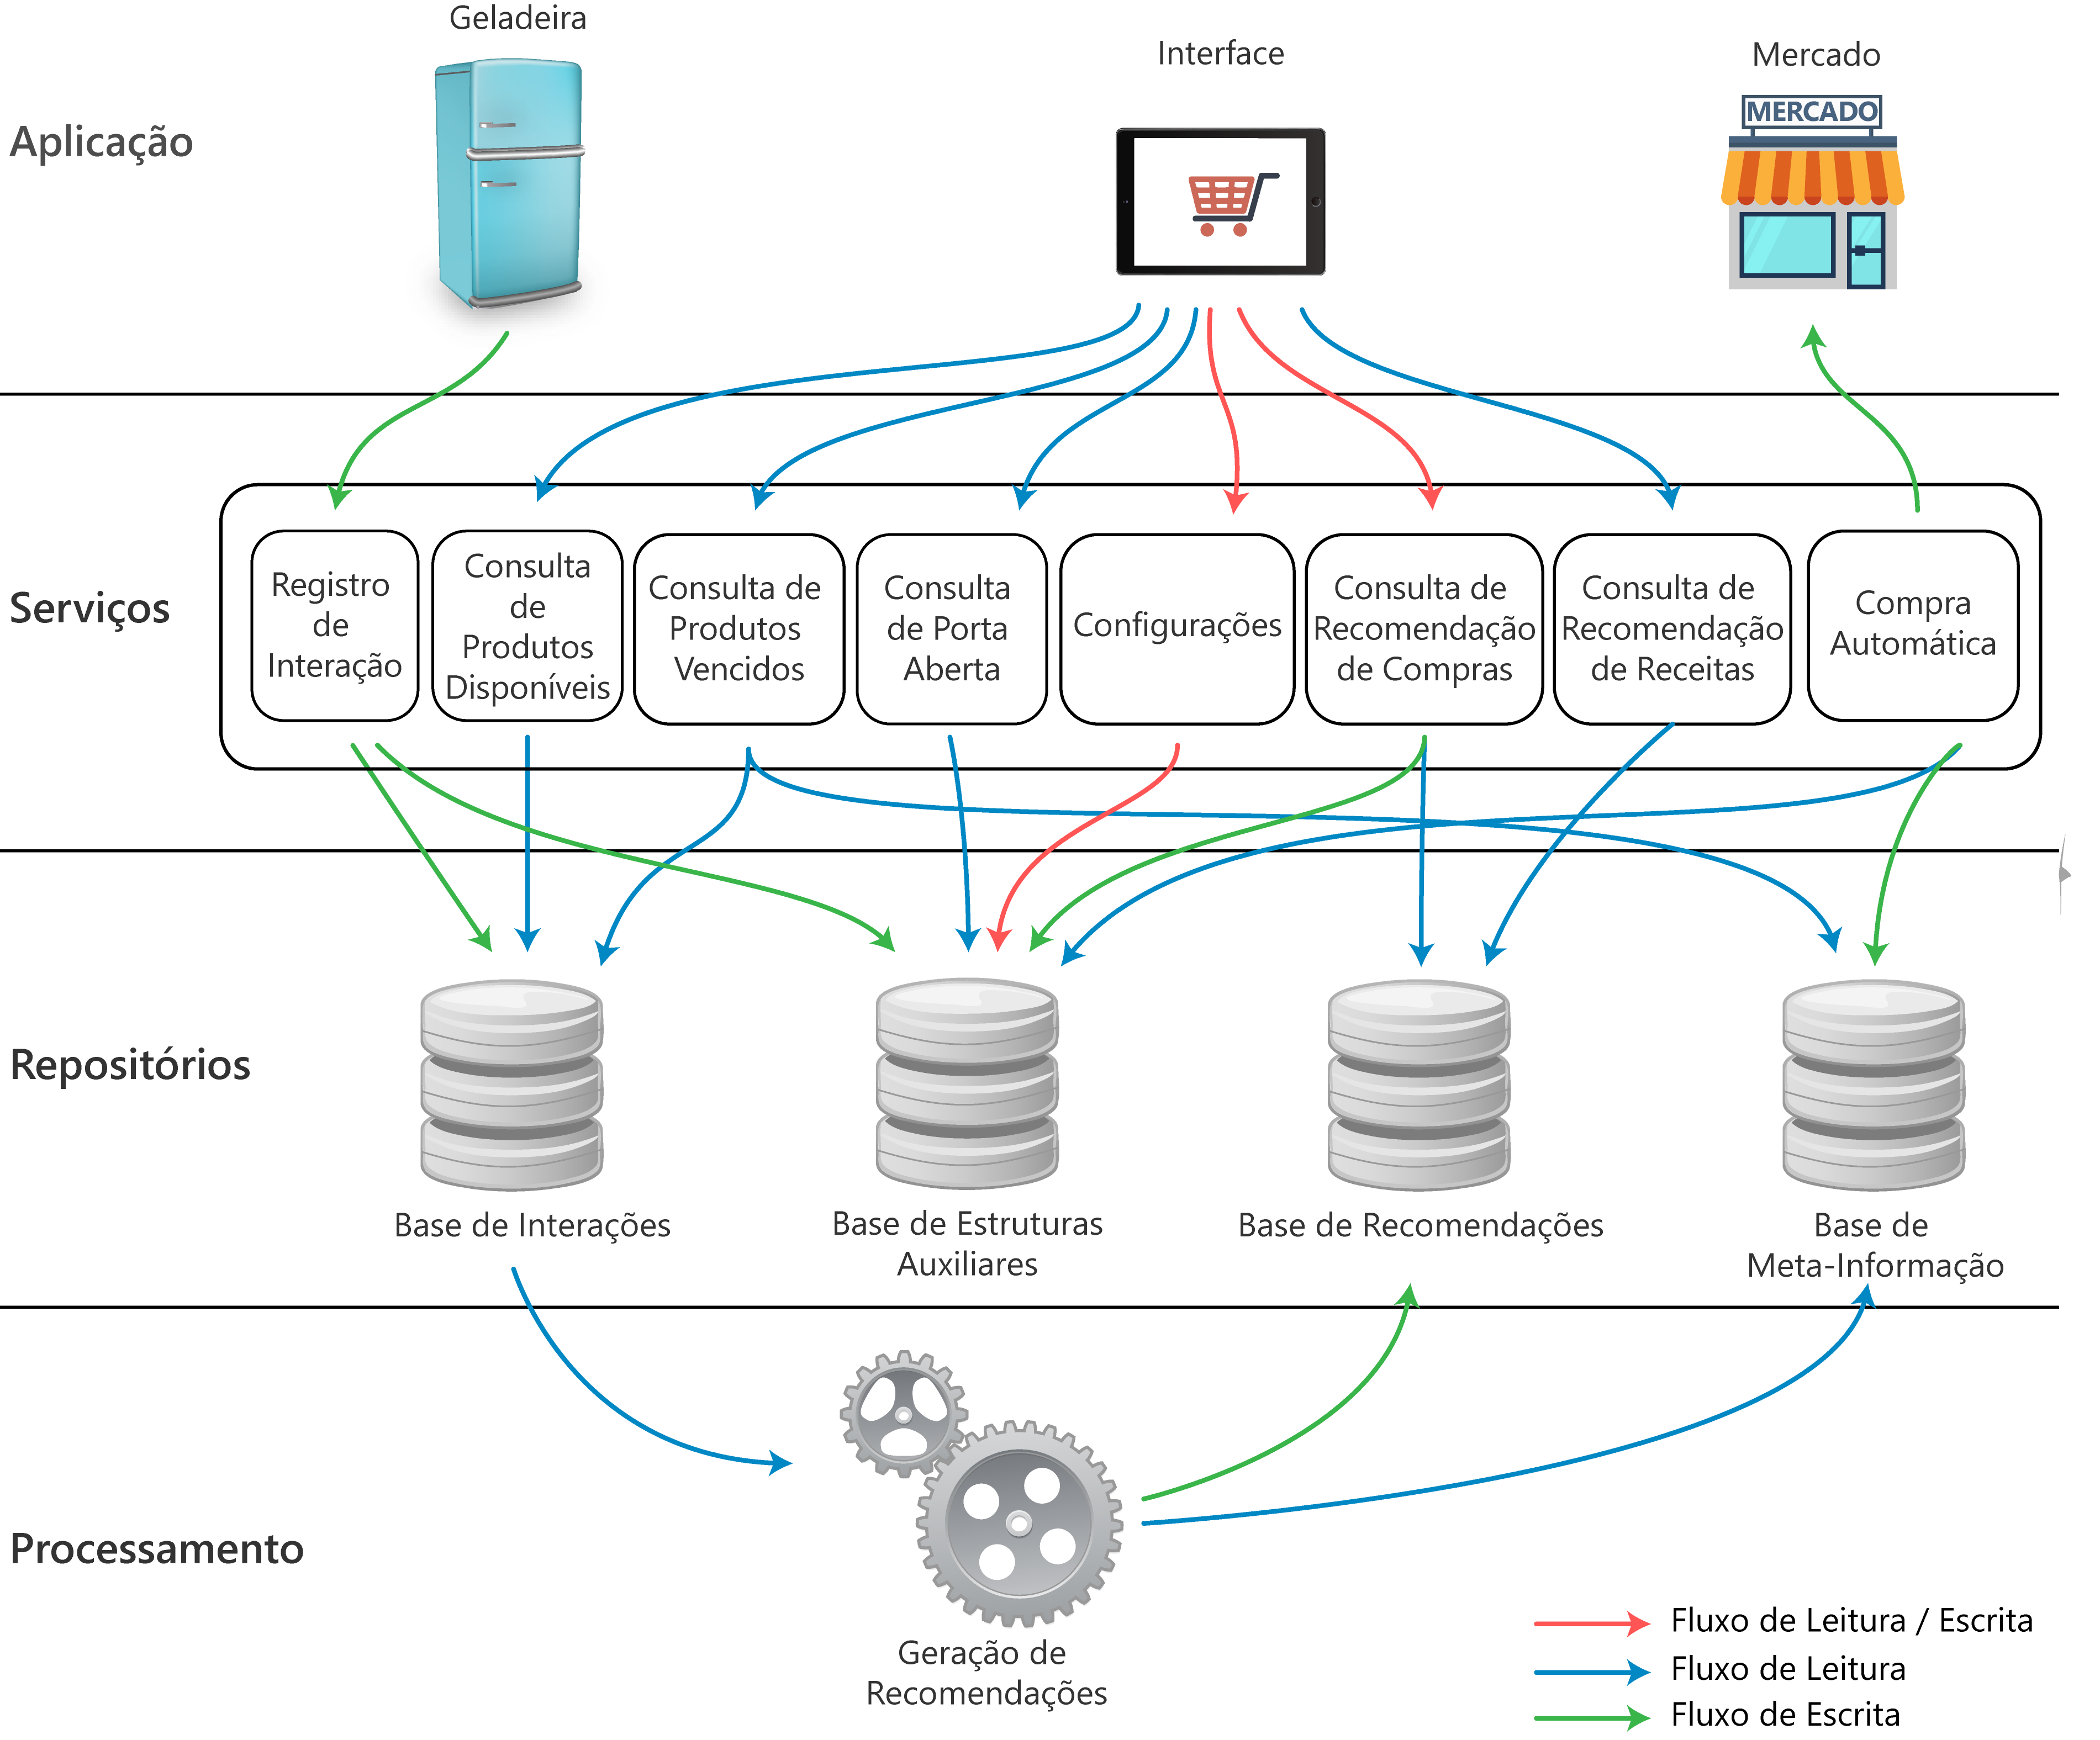
\includegraphics[width=0.92\textwidth]{modelo-logico}
    
    \footnotesize{Fonte: Elaborado pelo Autor}
\end{figure}
\nocite{Freepik2017} % fonte dos ícones

\subsection{Camada de Aplicação}

% Explanação sobre a camada

% Descrição da geladeira
%  - O que é
%  - Qual objetivo
%  - Porque

A camada de aplicação, como descrito, envolve os componentes externos ao sistema principal. O primeiro deles é a geladeira à qual se  responsabiliza por monitorar os produtos nela contidos. Deste modo, a cada interação do usuário com a geladeira é realizada uma varredura a fim de verificar o conjunto de produtos existentes. Em seguida, envia-se tais informações para o servidor através do serviço de registro de interação.

Outra funcionalidade da geladeira consiste na verificação da condição de fechamento da porta. Caso esteja aberta por um determinado período, a geladeira faz um registro na base de estruturas auxiliares através do serviço de registro de interação. Assim, o sistema é capaz de emitir um aviso ao usuário.

% Descrição da interface
%  - O que é
%  - Qual objetivo
%  - Porque

O componente seguinte é a interface de usuário, incorporada à porta da geladeira. Ela se responsabiliza por permitir ao usuário a interação com o eletrodoméstico. Assim, tem-se como funcionalidades deste componente: a listagem de produtos contidos, conjunto de produtos prestes a vencer, notificações de alerta caso o usuário esqueça a porta aberta, configurações personalizáveis e, por fim, recomendações de possíveis compras de produtos e receitas.

As recomendações podem ser exibidas automaticamente ou quando o usuário desejar. Assim, a aplicação realiza automaticamente a requisição e alerta o usuário através de uma notificação ou, ainda, o usuário solicita as recomendações através da interface.

% Descrição do mercado
%  - O que é
%  - Qual objetivo
%  - Porque

%O último componente da camada de aplicação é o mercado. 
%A partir deste será possível fazer verificações da existência de produtos da geladeira com prazo de validade expirados. 
%Além disso, permite que, 


%  é possível fazer consultas de promoções de itens que eventualmente serão disponibilizadas pelo mercado.

\subsection{Camada de Serviços}

A camada de serviços disponibiliza um conjunto de funcionalidades aos componentes da camada de aplicação, se comportando como meio de entrada do sistema principal. Assim, há um conjunto de serviços específicos disponibilizados conforme a Figura \ref{fig:c4_modelo_logico} e que serão descritos nos parágrafos seguintes.

% Explanação sobre a camada serviços

% Descrição do "Registro de interação"
%  - O que é
%  - Qual objetivo
%  - Porque
O serviço de registro de interação recebe informações dos itens contidos da geladeira além do alerta de porta aberta. Em seguida, registra-se tais informações na base de interações e de estruturas auxiliares, respectivamente.


% Descrição do "Consulta de Produtos Disponíveis"
%  - O que é
%  - Qual objetivo
%  - Porque

Já o serviço de consulta de produtos disponíveis pode ser requisitado pelo usuário através da interface. 
%A partir disto, será realizada uma busca na base de interações pelo último registro feito ao qual conterá os produtos existentes no momento.
Então, o conjunto de produtos contidos na geladeira é obtido a partir do último registro inserido na base de interações, já que este último mostra o estado mais recente da geladeira.

% Descrição do "Consulta de produtos vencidos"
%  - O que é
%  - Qual objetivo
%  - Porque

O serviço de consulta de produtos vencidos é acionado periodicamente pela interface. Desse modo, é efetuada uma busca pelo itens disponíveis na geladeira e o tempo que estão presentes, através da base de interações. Logo após, se realiza uma consulta na base de metainformação para determinar o período de validade (após aberto) de cada produto encontrado. A partir da comparação entre tempo de acondicionamento e prazo de expiração, sabe-se se o produto está vencido ou não. A estimativa é feita pois o prazo de validade transcrito nos produtos se reduz após sua abertura.

% Descrição do "Consulta de porta aberta"
%  - O que é
%  - Qual objetivo
%  - Porque
O serviço de consulta de porta aberta é requisitado pela interface de usuário periodicamente de forma automática. Como efeito da requisição, faz-se uma consulta à base de estruturas auxiliares a fim verificar a existência de um registro recente de porta aberta. O resultado é então encaminhado para a interface que alertará o usuário, caso necessário.

% TODO: O último registro diz se a porta está aberta ou não.

% Descrição do "Configurações"
%  - O que é
%  - Qual objetivo
%  - Porque

O serviço de configurações permite que o usuário personalize algumas características do funcionamento da geladeira. A primeira delas se refere ao mercado no qual as compras são realizadas. Além disso, é possível determinar quais produtos devem sempre estar disponíveis para consumo e qual a quantidade mínima necessária.

% Descrição do "Consulta de Recomendação de Compras"
%  - O que é
%  - Qual objetivo
%  - Porque

O serviço de consulta de recomendação de compras é requisitado pela interface periodicamente e também pelo usuário. Assim, quando é feita uma requisição, automática ou não, o serviço faz uma consulta à base de recomendações em busca de possíveis sugestões. O conjunto existente é então retornado para a interface que, por sua vez, indaga ao usuário se deseja realizar a compra e quais produtos, dentre os apresentados, deseja adquirir. A lista é retornada ao serviço que, então, faz o registro na base de estruturas auxiliares.

% Descrição do "Consulta de Recomendação de Receitas"
%  - O que é
%  - Qual objetivo
%  - Porque

O serviço de recomendação de receitas recebe uma requisição do usuário e faz uma consulta à base de recomendações. Caso existam receitas para recomendar, essas serão listadas ao usuário na interface sendo possível a escolha de qual receita se deseja visualizar.

% Descrição do "Compra automática"
%  - O que é
%  - Qual objetivo
%  - Porque

\subsection{Camada de Repositórios} \label{sec:camada-repo}

% Explanação sobre a camada
O conjunto de repositórios desta camada atuam na persistência de informações geradas pelos diversos componentes das camadas de aplicação e de processamento, sendo divididas em quatro bases: de interações, de estruturas auxiliares, de recomendações e de metainformação.
A primeira base é responsável, como descrito anteriormente, pelo registro de produtos acondicionados na geladeira. A partir disso, as consultas realizadas nessa base podem recuperar os itens constantes após cada interação do usuário.

A base de estruturas auxiliares contém informações que são utilizadas por mais de um serviço. Tais informações representam alertas de porta aberta, configurações e as listas de compras efetuadas pelo usuário. 

Já a base de recomendações armazena todas as sugestões de receitas e de compras de produtos que foram elaboradas pelo módulo de geração de recomendações e que serão apresentadas ao usuário.

A última base, de metainformação, contém informações referentes ao conteúdo dos produtos adquiridos e que são utilizadas pelo módulo de geração de recomendações e pelo serviço de verificação de produtos vencidos. Tais informações incluem características do produto, como código de barras, fabricante, informações nutricionais, categoria além do tempo estimado de validade. Além disso, inclui-se registros de receitas e suas respectivas informações, ou seja, ingredientes, e passos para o preparo destas.

\subsection{Camada de Processamento}

% Explanação sobre a camada
A camada de processamento contém os módulos de geração de recomendações, de compras automáticas e de sincronização de metainformação. O primeiro deles faz uso das informações armazenadas na base de interação e das características de cada item, mantidas na base de metainformações.

% Como vai receber do mercado informações de que tem itens em promoção.
As recomendações de receitas fazem uso da base de interações para ter conhecimento dos produtos contidos atualmente e de metainformações para resgatar as receitas e seus respectivos ingredientes. A partir disso, é feita uma comparação entre as bases. Caso alguma receita tenha a necessidade de itens que já estão presentes, essa será recomendada ao usuário. %Do contrário, caso apenas alguns itens estejam em falta, será sugerida, ao usuário, além da receita, a compra dos produtos faltantes.

Compras são sugeridas com base na quantidade existente de um certo produto. Assim, quando tal valor fica abaixo da quantidade mínima, determinada pelo usuário, é realizada a recomendação de compra do produto. No entanto, o mercado pode não ter à disposição o produto específico, mas pode conter similares. Neste caso, o sistema efetua uma busca por itens similares e solicita a aprovação do usuário para a compra deste, ao invés do original. Além disso, sugere-se novos itens, aos quais tenha apresentado interesse, que, por ventura, o mercado venha a disponibilizar.

O processo de compra é executado automaticamente quando há uma lista de compras pendente. Assim, a partir da verificação de tal pendência na base de estruturas auxiliares, a compra é requisitada ao mercado. 

Já o processo de sincronização de metainformações, periodicamente consulta o serviço de sincronização do mercado para verificar se há metainformações de produtos que foram adicionados ou alterados.

\subsection{Camada de Agente Externo}

O componente desta camada é o mercado. Através dele, torna-se possível verificar a disponibilidade de produtos e efetivar compras a partir da lista de produtos selecionados pelo usuário. Além disso, há a funcionalidade de sincronização de metainformação de produtos onde, para isso, o mercado disponibiliza um serviço possibilitando que a base de metainformação possa ser periodicamente atualizada. Essas informações são utilizadas posteriormente na recomendação de produtos e receitas.


%%%%%%%%%%%%%%%%%%%%%%%%%%%%%%%%%%%%%%%%%%%%%%%%%%%%%%%%%%%%%%%%%%%%%%%%%%%%%%%%%%%%%%%%%%%%%%%%%%%%%%%%%
%                                                                                                       %
%                                              MODELO FÍSICO                                            %    
%                                                                                                       %
%%%%%%%%%%%%%%%%%%%%%%%%%%%%%%%%%%%%%%%%%%%%%%%%%%%%%%%%%%%%%%%%%%%%%%%%%%%%%%%%%%%%%%%%%%%%%%%%%%%%%%%%%

\section{Modelo F\'isico}
% Descrição da geladeira
%  - O que é
%  - Qual objetivo
%  - Porque

% Explicar o que há dentro de cada componente lógico
% Se preciso desenhar a arquitetura interna do componente
% Por exemplo a geladeira, vai ter muitas coisas dentro que devem ser explicitadas

A modelagem física deste trabalho é apresentada na Figura \ref{fig:c4_modelo_fisico}. Nas seções a seguir serão detalhados os diversos componentes do sistema, em relação aos aspectos internos.


\begin{figure}[H]
    \caption{Modelo físico}
    \label{fig:c4_modelo_fisico}
    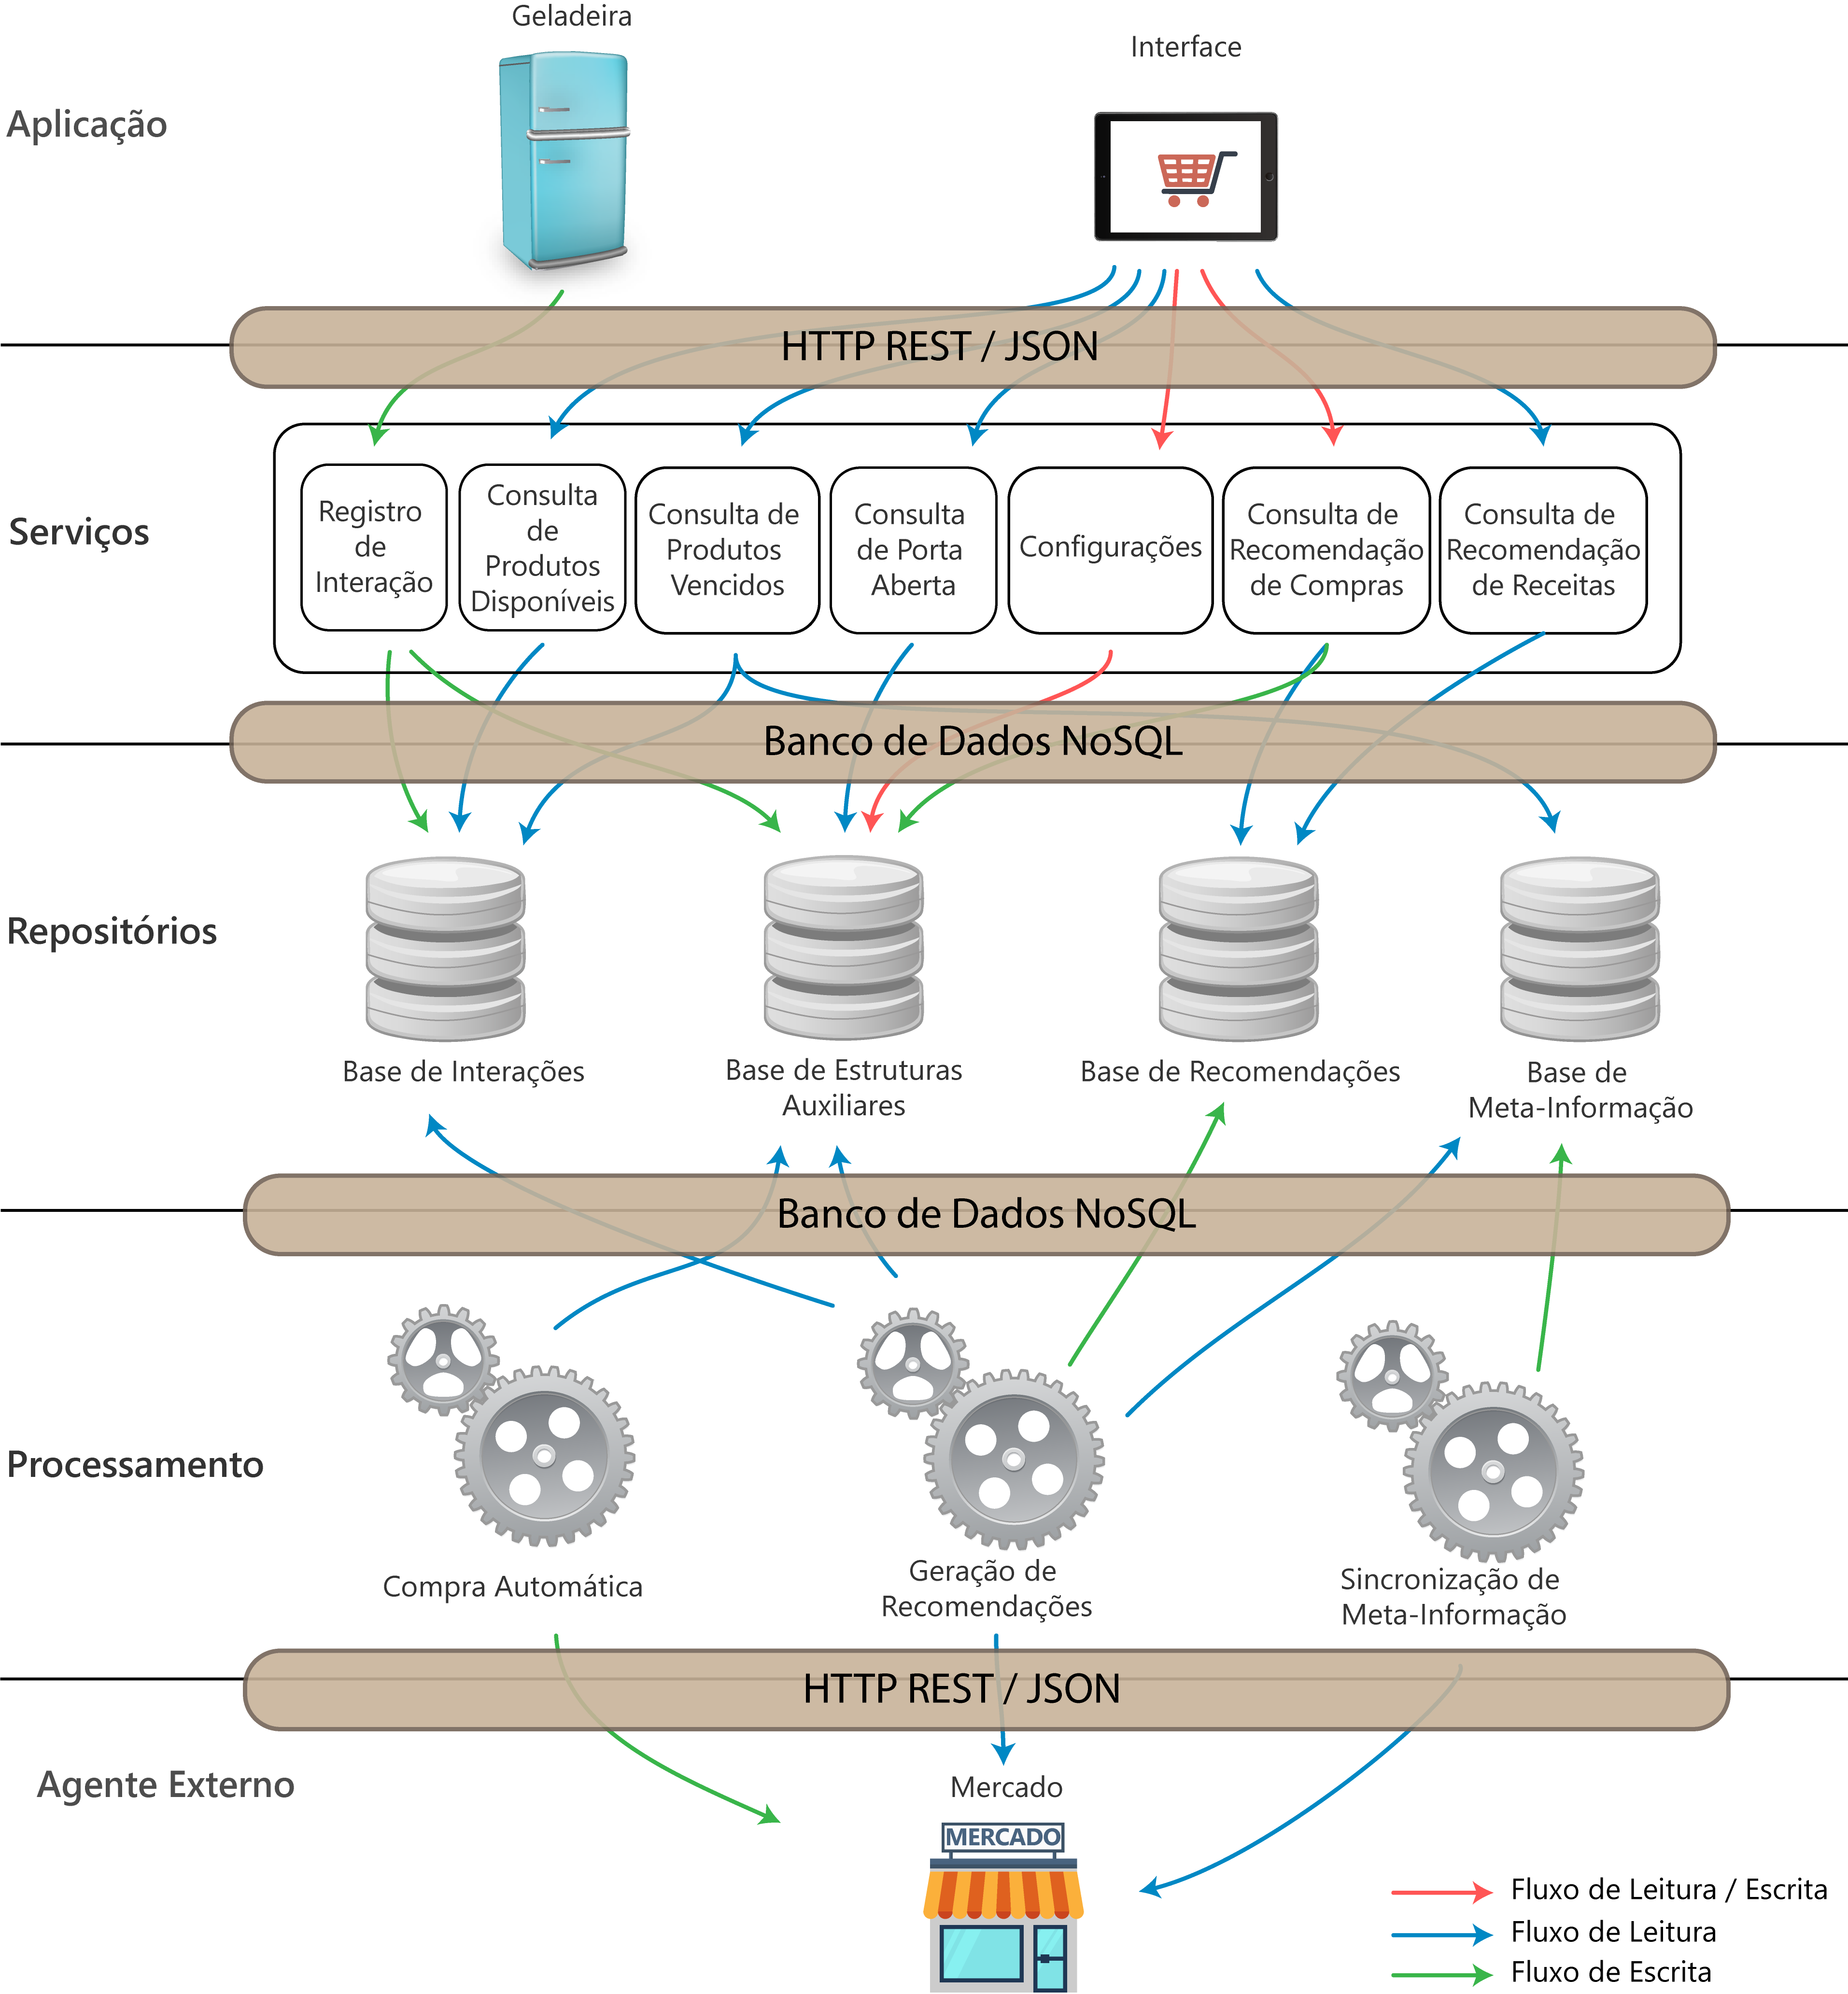
\includegraphics[width=0.8\textwidth]{c4_modelo-fisico.png}
    
    \footnotesize{Fonte: Elaborado pelo Autor}
\end{figure}

%%%%%%%%%%%%%%%%%%%%%%%%%%%%%%%%%%%%%%%%%%%%%%%%%%%%%%%%
\subsection{Camada de Aplicação}

\ProximoForaDoSumario 
\subsubsection{Geladeira}

A geladeira, presente no modelo lógico da Figura \ref{fig:c4_modelo_logico}, foi construída de acordo com a Figura \ref{fig:cap4_estr_geladeira}. Assim, observa-se três componentes principais: os leitores de etiquetas MFCR522 para RFID e NFC, o sensor de fechamento para a porta e a placa Raspberry PI\textsuperscript{\textregistered}\footnote{https://www.raspberrypi.org} 3 Modelo B. O primeiro deles, o conjunto de leitores, responsabiliza-se por efetuar varreduras de etiquetas NFC próximas a cada leitor quando for requerido. A partir disso, os dados lidos, referentes aos produtos, são transferidos para o Raspberry PI que, por sua vez, os transfere para o serviço de registro de interação. Os dados das etiquetas se encontram no formato \textit{Electronic Product Code} (EPC), no qual, identifica-se o fabricante, a classe do produto e a instância do produto a partir de um número de 96 bits, de forma semelhante ao código de barras presente nos produtos \cite{GS1BR2017}. Vale destacar que as etiquetas utilizadas nesse trabalho operam na faixa HF de 13,56 MHz e foram configuradas no formato NDEF.

\begin{figure}[htb]
    \caption{Estrutura interna da geladeira}
    \label{fig:cap4_estr_geladeira}
    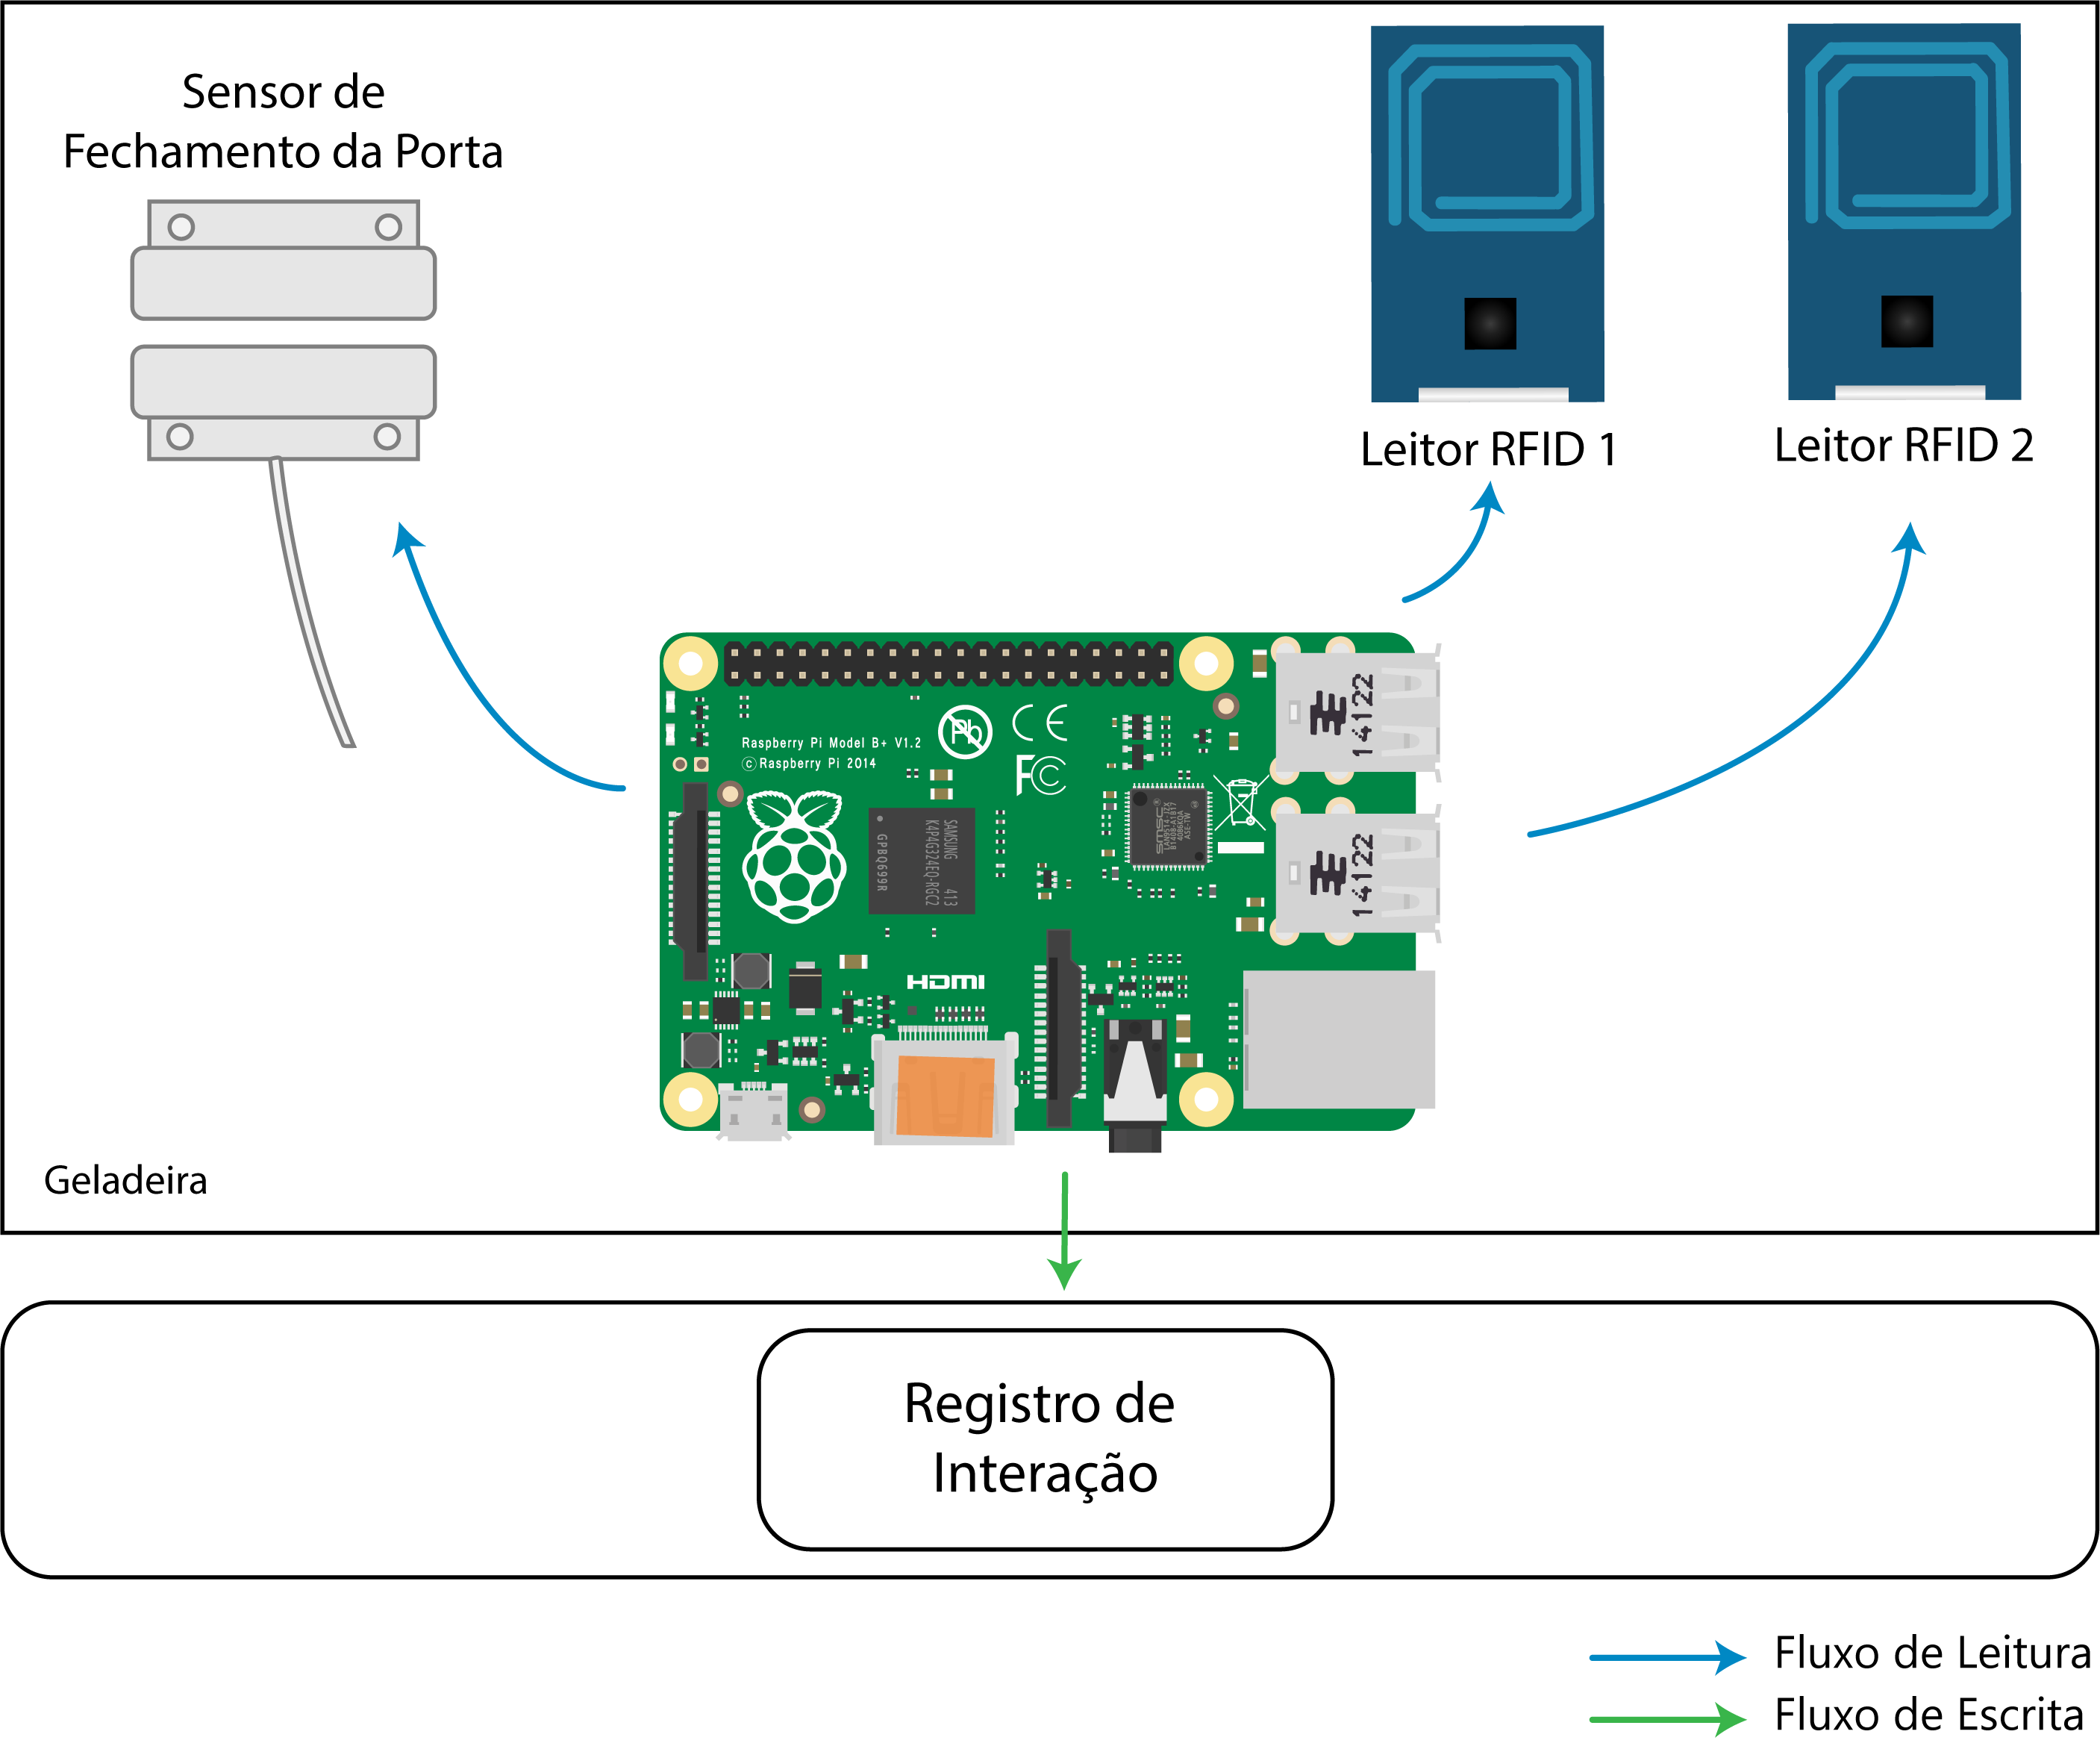
\includegraphics[width=\textwidth]{figuras/c4_modelo-logico-hardware.png}
    
    \footnotesize{Fonte: Elaborado pelo Autor}
\end{figure}

O sensor de fechamento de porta, por outro lado, é responsável por determinar quando ações devem ocorrer. O seu funcionamento envolve dois componentes: o primeiro é dotado de um imã e o outro contém um mecanismo que é influenciado pela presença ou não do ímã. Assim, quando estes se aproximam, indica-se o fechamento da porta. Haverá, deste modo, um curto-circuito entre os terminais do mecanismo. Por outro lado, quando afastados indica-se abertura, determinando portanto, um circuito aberto.



%Considerando-se, primeiramente, o evento de abertura da porta, caso o usuário não feche a porta durante um determinado período de tempo
Considerando que inicialmente a porta está fechada. Em um dado momento, o usuário abre a porta. Caso esta não seja fechada durante um determinado período de tempo, será feita uma requisição para o serviço de registro de interação indicando a situação. Caso contrário, ou seja, a porta esteva aberta e é fechada dentro do período estipulado, realiza-se uma varredura dos produtos e, em seguida, uma requisição é enviada ao serviço para que se efetue o registro de interação.

Por fim, o último componente, o Raspberry PI, opera como um centro de controle, onde obtém dados do sensor de fechamento para, então, comandar leituras de etiquetas e/ou fazer requisições descritas anteriormente.

Para a comunicação entre os três componentes fez-se uso de dois protocolos específicos: a \textit{Serial Peripheral Interface} (SPI) e \textit{Hypertext Transfer Protocol} (HTTP) com \textit{Representational State Transfer} (REST). O primeiro deles foi empregado na comunicação entre os leitores RFID e o Rasbpberry, já o segundo, para a troca de informações entre o Raspberry e o serviço de registro. Por fim, a comunicação com o sensor de fechamento ocorre através de sinais digitais.

Como parte do processo de implementação, uma estrutura em madeira foi construída a fim de simular a interação. O resultado pode ser observado na Figura \ref{fig:cap4_imagem_estrutura}. Assim, apesar da aparência rústica, observa-se três níveis: o primeiro, inferior, abriga o Raspberry, já o segundo e terceiro abrigam os leitores e os produtos.

%%%%%%%%%% FIGURA X - Estrutura da geladeira  %%%%%%%%
\begin{figure}[H]
    \caption{Estrutura externa da geladeira}
    \label{fig:cap4_imagem_estrutura}
    \includegraphics[width=0.51\textwidth]{figuras/cap4_imagem_estrutura.png}
    
    \footnotesize{Fonte: Elaborado pelo Autor}
\end{figure}


\ProximoForaDoSumario 
\subsubsection{Interface de Usuário}

Como já descrito, a interface de usuário destina-se à interação entre usuários e a geladeira. Assim, conforme Figura \ref{fig:cap3_app_mainpage}, as funcionalidades ficam disponíveis em um tela principal e podem ser acessadas de acordo com a necessidade do usuário ou em momentos em que notificações forem disparadas.

\begin{figure}[htb]
    \caption{Página principal da interface}
    \label{fig:cap3_app_mainpage}
    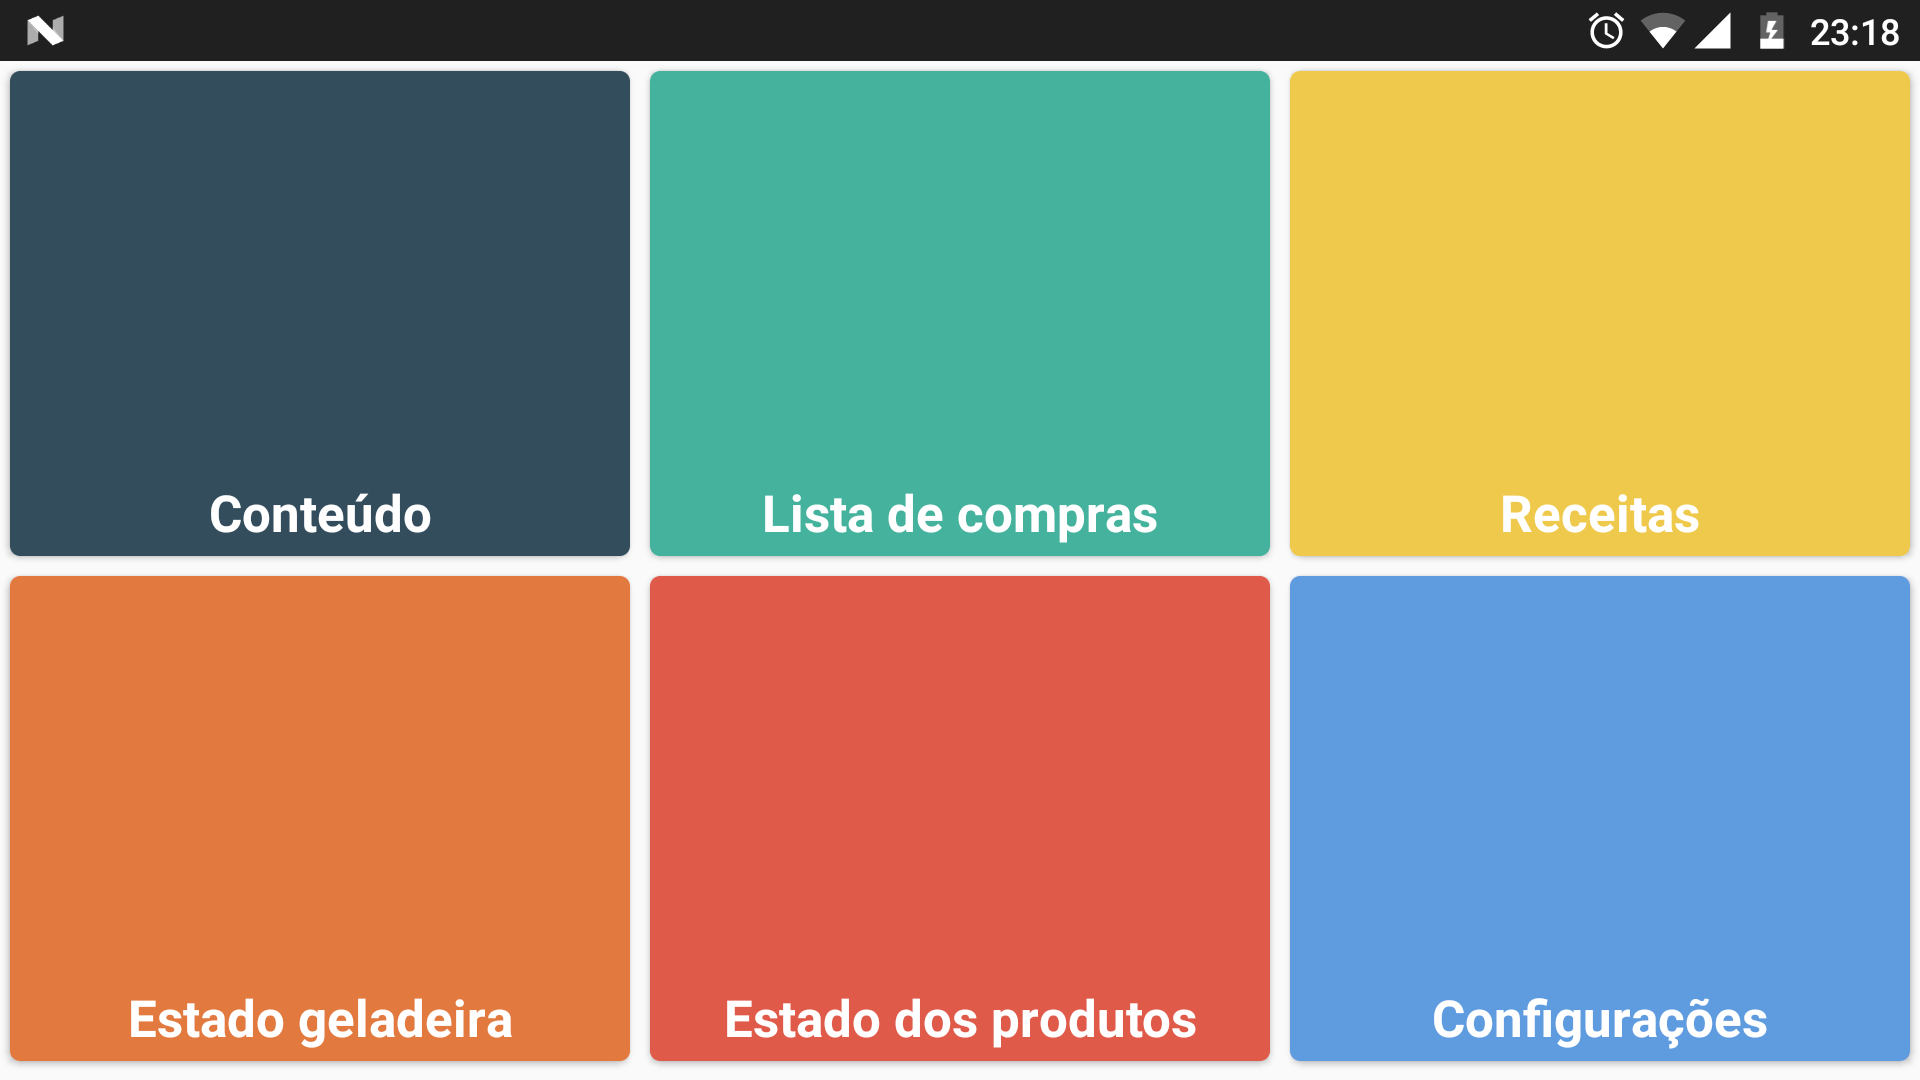
\includegraphics[width=0.8\textwidth]{figuras/cap4_app_mainpage.png}
    
    \footnotesize{Fonte: Elaborado pelo Autor}
\end{figure}

A primeira das funcionalidades, de listagem de conteúdo, é exibida como um conjunto de produtos com as respectivas informações de descrição, fabricante e quantidade disponível, conforme Figura \ref{fig:cap4_listagem_de_produtos}.

\begin{figure}[htb]
    \caption{Listagem de produtos}
    \label{fig:cap4_listagem_de_produtos}
    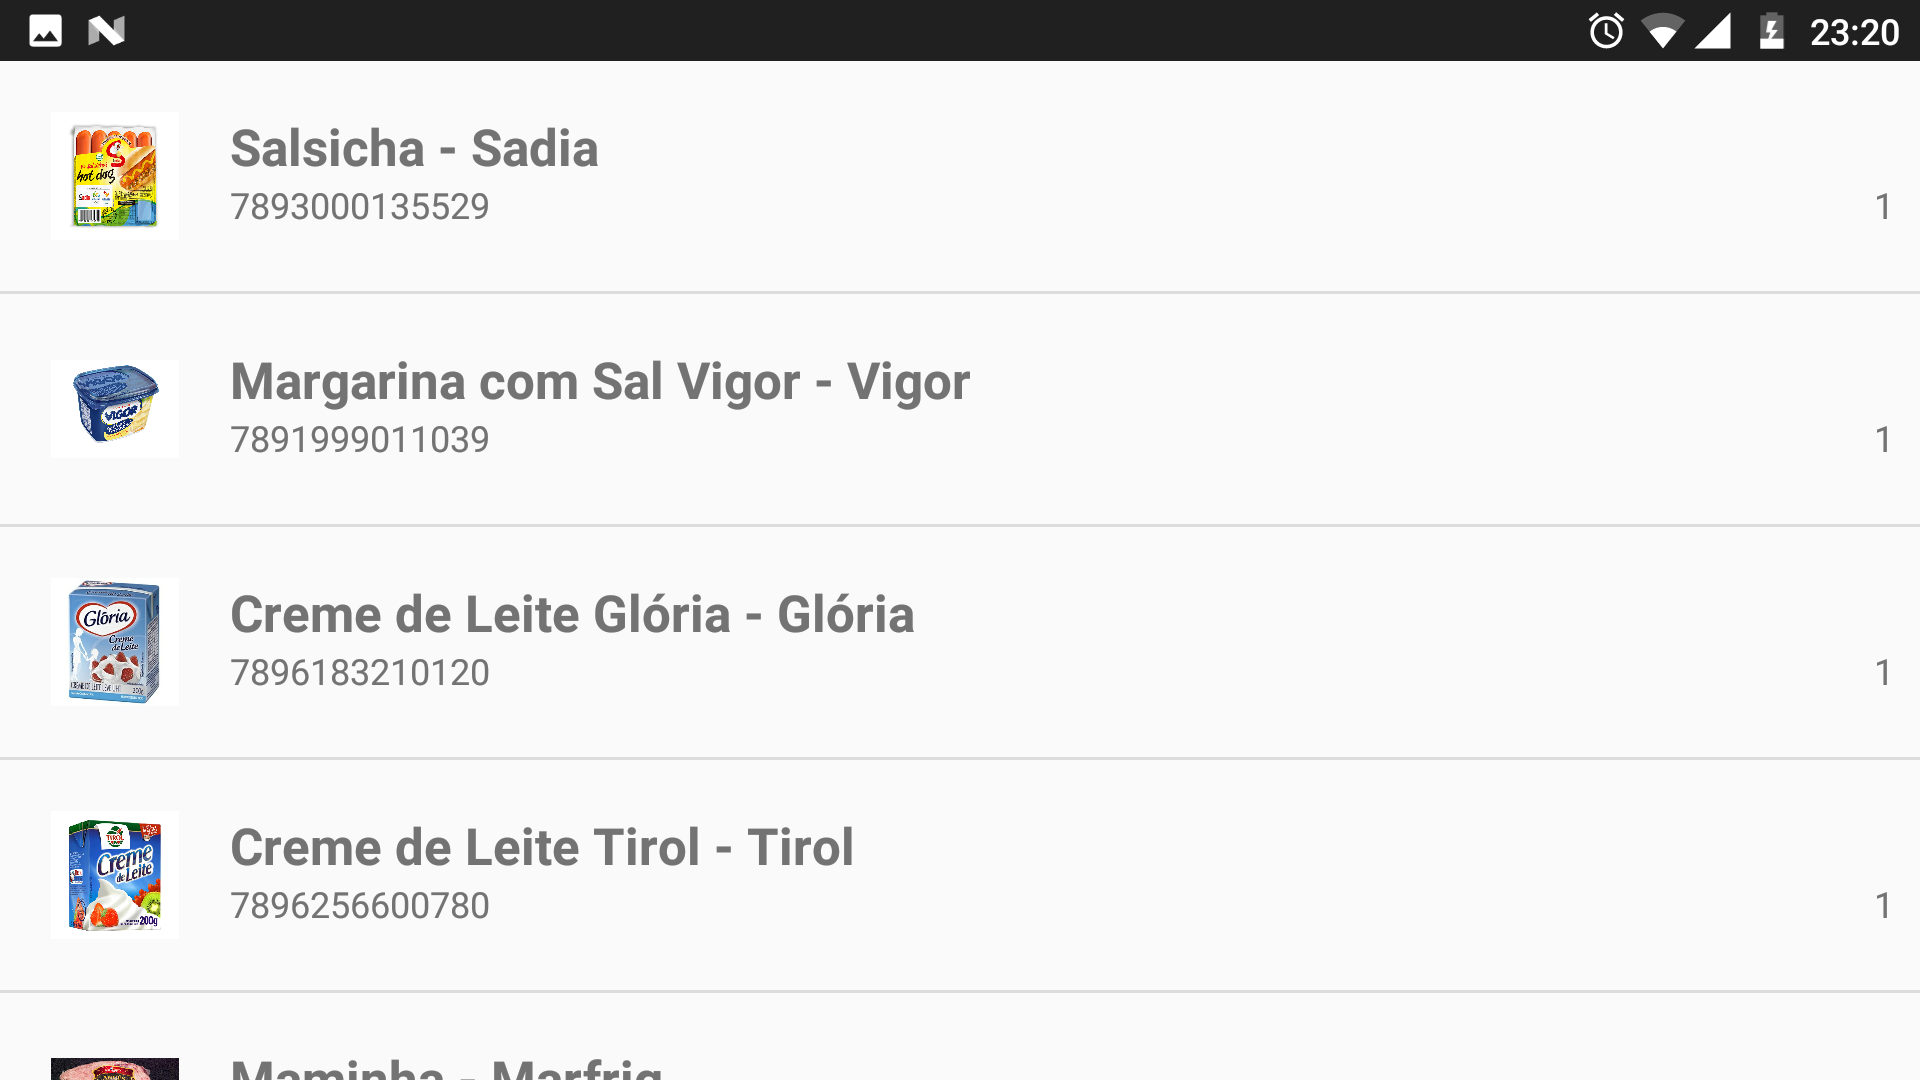
\includegraphics[width=0.8\textwidth]{figuras/cap4_listagem_de_produtos.png}
    
    \footnotesize{Fonte: Elaborado pelo Autor}
\end{figure}

A próxima função permite que o usuário visualize receitas recomendadas. Assim, inicialmente será listado um conjunto de receitas selecionados pelo sistema. Em seguida, é possível visualizar os detalhes de qualquer uma delas, como ingredientes e passos para o preparo, conforme Figura \ref{fig:cap4_exibicao_receita}.

\begin{figure}[htb]
    \caption{Exibição de detalhes de uma receita}
    \label{fig:cap4_exibicao_receita}
    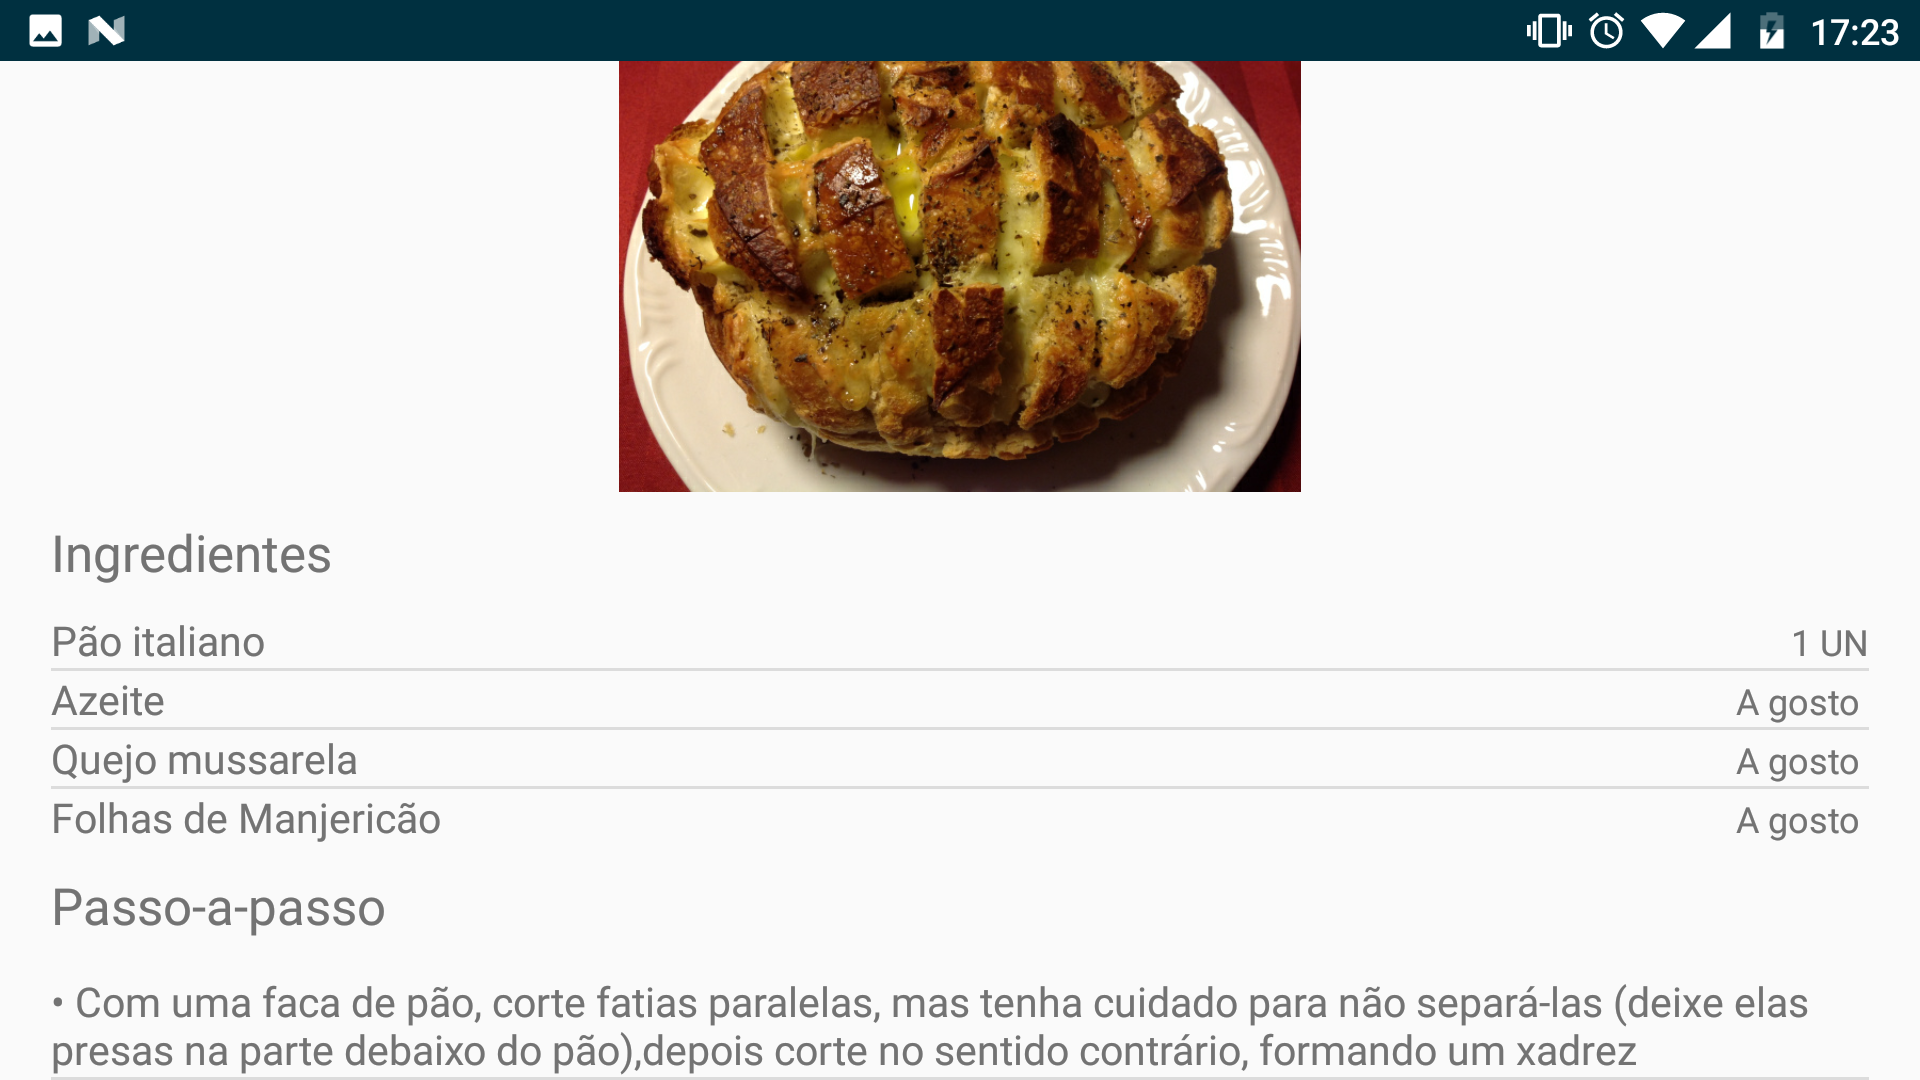
\includegraphics[width=0.8\textwidth]{figuras/cap4_exibicao_receita.png}
    
   \footnotesize{Fonte: Elaborado pelo Autor}
\end{figure}

A última funcionalidade implementada é a exibição do estado da geladeira, ou seja, se está aberta ou fechada no momento. Acessando a respectiva opção no menu da Figura \ref{fig:cap3_app_mainpage} uma nova tela é aberta e o estado atual é exibido. Outra forma na qual a aplicação permite ter conhecimento do estado da geladeira é através de notificações que alertam em caso de a porta estar aberta durante muito tempo.

Toda a interface de usuário foi desenvolvida a partir de um aplicação para a plataforma móvel Android\textsuperscript{\textregistered}.

%\subsubsection{Mecanismo de Geração de Recomendações (\textit{Rascunho})}

%Para a geração de recomendações de compras de produtos, tem-se duas situações: de acordo com os produtos que acabaram e de acordo com o que pode gostar. No primeiro caso, utiliza-se um híbrido entre filtragem colaborativa e baseada em conteúdo. Assim, será verificada a ausência de produtos que o usuário acha importante e a compra dos respectivos produtos será recomendada. Caso o produto em específico não esteja disponível, será avaliada a disponibilidade de produtos semelhantes e que outros usuários com gostos semelhantes também compraram e estes serão sugeridos. Já no segundo caso, será feito uma simples filtragem colaborativa onde, eventualmente, serão sugeridos produtos de acordo com os gostos do usuário em comparação com os demais.

%Para a geração de recomendações de receitas, tem-se duas situações: de acordo com o que tem disponível e de acordo com o que gosta. No primeiro caso, será feito uma busca por receitas que podem ser preparadas com os produtos contidos na geladeira a partir de abordagem baseada em conteúdo. Já a segunda, será feita a partir dos gostos do usuário considerando os dos outros e o conteúdo dos itens que mais gosta, ou seja, as receitas devem conter os produtos que o usuário mais gosta.

%%%%%%%%%%%%%%%%%%%%%%%%%%%%%%%%%%%%%%%%%%%%%%%%%%%%%%%%
\subsection{Camada de Serviços} \label{ssec:c5_camada_servicos}

% Objetivo
Como descrito anteriormente, a camada de serviços atua como porta de entrada do sistema para os componentes da camada de aplicação. 
% Tecnologias
Conforme demonstrado na Figura \ref{fig:c4_modelo_fisico}, utiliza-se, sobre o HTTP, o REST, um estilo arquitetural que opera como um modelo abstrato da arquitetura da \textit{Web}. Em outras palavras, qualquer informação contida em um servidor pode ser abstraída como um recurso. Além disso, cada recurso é identificado por um \textit{Uniform Resource Identifier } (URI) e o acesso a esse recurso ocorre por meio de métodos HTTP, como o GET e o POST \cite{Fielding2000}.

% JAX-WS
Para a implementação dos serviços REST utilizou-se a linguagem Java a partir do \textit{ Integrated Development Environment} (IDE) Eclipse \textit{Java Enterprise Edition} (JEE) com a especificação \textit{Java API for XML Web Services} (JAX-WS) para a referida linguagem.

% Formato de Requisições
Como exemplos, é possível apresentar os serviços de registro de interação e de consulta do estado da porta, conforme Quadro \ref{fig:cap4_service-register} e Quadro \ref{fig:cap4_service-status-door}, respectivamente.

\begin{quadro}[htb]
    \caption{Serviço de registro de interação}
    \label{fig:cap4_service-register}
   \frame{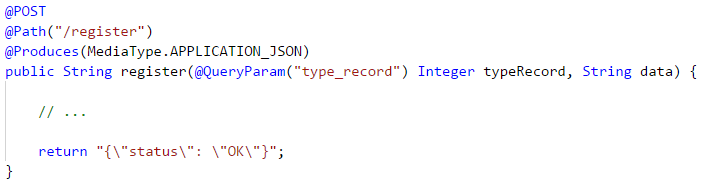
\includegraphics[width=\textwidth]{cap4_service-register}}
    
    \footnotesize{Fonte: Elaborado pelo Autor}
\end{quadro}


% \begin{figure}
%  \caption{Serviço de registro de interação}
%        \label{fig:cap4_service-register}
%        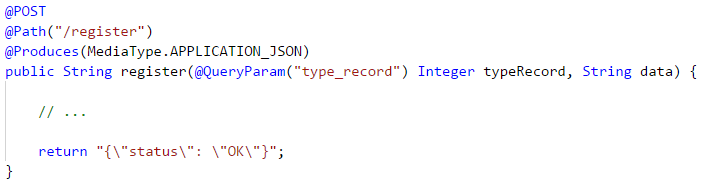
\includegraphics[width=\textwidth]{cap4_service-register}
%        
%        \footnotesize{Fonte: Autor}
%    \end{figure}


\begin{quadro}[htb]
    \caption{Serviço de consulta de estado de porta}
    \label{fig:cap4_service-status-door}
    \frame{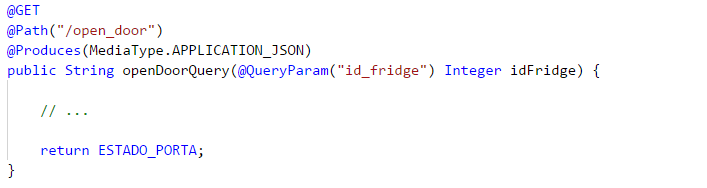
\includegraphics[width=\textwidth]{cap4_service-status-door}}
    
    \footnotesize{Fonte: Elaborado pelo Autor}
\end{quadro}


Como descrito, a estrutura de um serviço conta com um método HTTP para ser acessado. Nos exemplos, utiliza-se os métodos \texttt{POST} e \texttt{GET}, respectivamente. Além disso, para cada serviço atribuiu-se um endereço, sendo eles, \texttt{/register} e \texttt{/open\_door}, nessa ordem. 

% A estrutura de um serviço, como descrito, é composto pelo método pelo qual é acessado sendo nos serviços de exemplo, \texttt{POST} e \texttt{GET}, respectivamente. Além disso, é atribuído um endereço em específico para cada serviço sendo, \texttt{/register} e \texttt{/open\_door}, nessa ordem. 

É possível especificar a interação com o serviço a partir de parâmetros, aos quais variam de acordo com o método HTTP utilizado. Assim, é possível informar parâmetros na URL na própria requisição HTTP, tanto no POST quanto no GET, ou apenas no corpo da mesma, no caso do POST.

Por fim, cada serviço poderia ser acessado pelas seguintes URIs.

\begin{itemize} \parskip -4pt
    \item \texttt{http://ipserver:8080/context/register?type\_record=1}
    \item \texttt{http://ipserver:8080/context/open\_door?id\_fridge=1}
\end{itemize}

% MongoDB
A interação dos serviços com as bases de repositórios, por outro lado, ocorre por meio de classes Java disponibilizadas pelo próprio mecanismo de armazenamento, ou seja, classes do MongoDB\textsuperscript{\textregistered}\footnote{https://www.mongodb.com}.

%\subsubsection{Registro de Interação}
%\subsubsection{Consulta de Produtos Disponíveis}
%\subsubsection{Consulta de Produtos Vencido}
%\subsubsection{Consulta de Porta Aberta}
%\subsubsection{Configurações}
%\subsubsection{Consulta de Recomendações de Compras}
%\subsubsection{Consulta de Recomendações de Receitas}


%%%%%%%%%%%%%%%%%%%%%%%%%%%%%%%%%%%%%%%%%%%%%%%%%%%%%%%%
\subsection{Camada de Repositórios}

As bases de dados nesse trabalho estão relacionadas ao servidor principal de serviços e recomendação. Conforme a Figura \ref{fig:c4_modelo_fisico}, tem-se quatro bases de dados: de interações, estruturas auxiliares, recomendações e metainformação. Tais bases promovem suporte para todas as funcionalidades do sistema, desde o registro de interações até a recomendação de produtos. 

A tecnologia utilizada para implementação dos repositórios baseia-se no conceito de banco de dados não relacionais, como o NoSQL. Tem-se como principal característica, nesse conceito, o não suporte ao modelo relacional para alcance de desempenho ou confiabilidade. O intuito desse tipo de banco de dados é ser utilizado em aplicações de grande escala, nas quais supera o desempenho de bancos relacionais. Os dados são registrados em coleções, que não restringem os tipos de dados armazenados. Consequentemente, é possível, por exemplo, registrar em uma mesma coleção cadastros de usuários e de fornecedores. \cite{Boicea2012}. 

Neste trabalho optou-se pelo MongoDB\textsuperscript{\textregistered}, um sistema de banco de dados NoSQL baseado em documentos, ao qual o armazenamento decorre no formato \textit{JavaScript Object Notation} (JSON), um formato baseado em chave e valor. 

O sistema desenvolvido neste trabalho possui um conjunto expressivo de interações provenientes dos dispositivos que o compõem, sendo que em um ambiente real resultaria em um número expressivo de inserções e recuperações de informação. Por isso, na implementação utilizou-se o conceito de base de dados NoSQL.

Nas seções que seguem, os repositórios serão detalhados em seus aspectos internos, como tipos de dados armazenadas, a origem da necessidade destes e em que momento são utilizados.

\ProximoForaDoSumario 
\subsubsection{Base de Interações}

Como descrito na Seção \ref{sec:camada-repo}, essa camada é responsável pelo registro das interações de usuários com produtos. A cada registro, ter-se-á um conjunto de códigos EPC de itens atuais, além da identificação da geladeira e o \textit{timestamp}, ou seja, o momento no qual ocorreu a interação. O Quadro \ref{fig:cap4_base-int_json} demonstra um exemplo de registro que é inserido na base.

\begin{quadro}[htb]
    \caption{Registro na base de interações}
    \label{fig:cap4_base-int_json}
    \frame{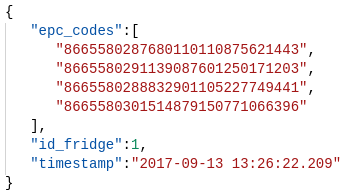
\includegraphics[width=0.45\textwidth]{cap4_base-int_json}}
    
    \footnotesize{Fonte: Elaborado pelo Autor}
\end{quadro}

Nota-se, pelo Quadro \ref{fig:cap4_base-int_json}, que haviam quatro itens na geladeira no dia 13 de setembro de 2017 à 13h26. No entanto, não é claro quais produtos estão contidos. Para tanto, operações de deslocamento de bit são realizadas sobre o código EPC revelando, desse modo, o fabricante, o produto e o número de série da instância. O Quadro \ref{fig:cap4_epc} exibe estrutura de um código EPC.

\begin{quadro}[htb]
    \caption{Estrutura de um código EPC}
    \label{fig:cap4_epc}
    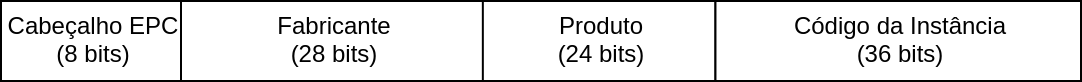
\includegraphics[width=\textwidth]{cap4_epc}
    
    \footnotesize{Fonte: Elaborado pelo Autor}
\end{quadro}

Esse tipo de registro é a principal fonte de informação sobre os hábitos dos usuários, uma vez que explicita os produtos com os quais mais se tem contato, bem como os horários em que isso ocorre. A partir dessas informações, é possível calcular as recomendações.


\ProximoForaDoSumario 
\subsubsection{Base de Estruturas Auxiliares}  \label{sssec:base_est-aux}

A base de estruturas auxiliares tem como principal objetivo intermediar a comunicação entre serviços e processos que fazem parte da camada de processamento. Assim, ela contém diversos tipos de registros, sendo eles, de estado da porta, configurações de cada geladeira e listas de compras pendentes.

O primeiro dos registros, informa qual o último estado registrado por uma determinada geladeira, ou seja, aberto ou fechado. Assim, tal informação será requisitada pela interface, através do serviço de consulta de porta, e alertará o usuário caso necessário. O Quadro \ref{fig:cap4_aux_setting}, demonstra um registro de estado da porta.

\begin{quadro}[htb]
    \caption{Estrutura de um registro de estado da porta}
    \label{fig:cap4_aux_setting}
    \frame{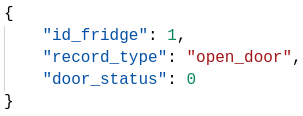
\includegraphics[width=0.35\textwidth]{cap4_aux_setting}}
    
    \footnotesize{Fonte: Elaborado pelo Autor}
\end{quadro}

Como é visível no Quadro \ref{fig:cap4_aux_setting}, três informações são guardadas: a identificação da geladeira, o tipo de registro que será inserido, ou seja, estado da porta, e o estado em si. Segundo a implementação, ``0'' significa porta aberta e, ``1'', fechada.

O segundo tipo de registro, de configurações, mantém um conjunto de parâmetros específicos de cada geladeira, conforme Quadro \ref{fig:cap4_settings}. 
%Esses parâmetros se referem ao serviço do mercado no qual às compras são realizadas e metainformações de produtos e receitas são resgatadas; ao tempo para que a porta da geladeira deve permanecer aberta antes que a interface notifique o usuário; ao período mínimo entre compras automáticas e os produtos que o usuário deseja que estejam sempre disponíveis. As demais informações se referem à identificação da geladeira, bem como o tipo de registro, nesse caso, de configurações.
Tais parâmetros incluem os dados do servidor do mercado escolhido e o tempo mínimo necessário que deve decorrer até que o usuário seja alertado que deixou a porta aberta. Além disso, inclui-se o intervalo de tempo em que ocorrem as compras automáticas e, por fim, a lista de produtos que são considerados essenciais.

As informações referentes ao mercado são utilizadas pelos processos do sistema. Já informações de tempo de notificação são requisitados pela interface através do serviço de configurações. Por outro lado, o tempo mínimo entre compras é requisitado pelo processo de compras automáticas. Por fim, a lista de produtos requeridos pelo usuário é utilizada pelo processo de recomendação na sugestão de novas compras.

\begin{quadro}[htb]
    \caption{Estrutura de um registro de configurações}
    \label{fig:cap4_settings}
    \frame{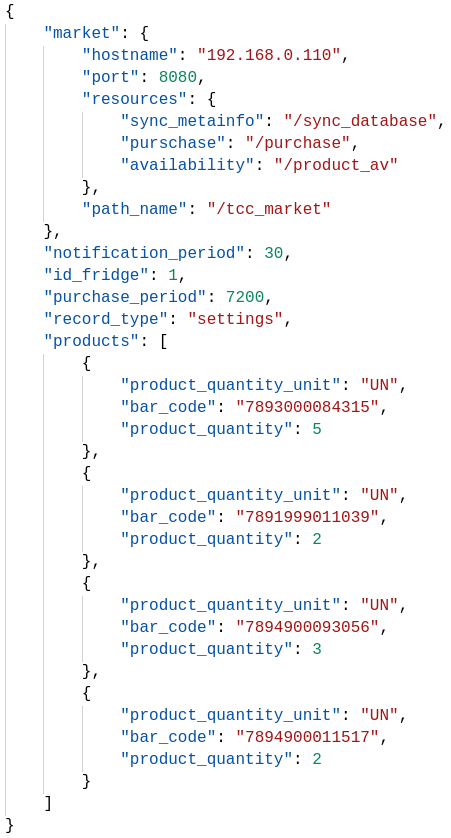
\includegraphics[width=0.5\textwidth]{cap4_settings}}
     
    \footnotesize{Fonte: Elaborado pelo Autor}
\end{quadro}

A terceira categoria de registros se refere às listas de compras definida pelo usuário. Neste caso, tem-se informações de identificação da geladeira, o momento no qual ao registro foi feito, bem como a lista de produtos e suas respectivas quantidades. Assim, tal lista será, posteriormente, analisada e efetivada pelo processo de compra automática.


% TODO: COLOCAR FIGURA DA LISTA DE COMPRAS AQUI.

%-----------------------------------------------------------%
\ProximoForaDoSumario 
\subsubsection{Base de Metainformação} \label{sssec:metainfo}

% META INFO DE PRODUTOS

Os produtos disponibilizados pelo mercado possuem suas informações armazenadas nessa base de dados. Desta forma, o sistema terá acesso a preços, códigos de barras, informações nutricionais, entre outros. Assim, torna-se possível utilizar tais informações em recomendações como, por exemplo, produtos similares a um em específico. 

A estrutura do registro de um produto em específico é demonstrada no Quadro \ref{fig:cap4_metainfo}.

\begin{quadro}[htb]
    \caption{Estrutura de um registro de metainformação de produto}
    \label{fig:cap4_metainfo}
    \frame{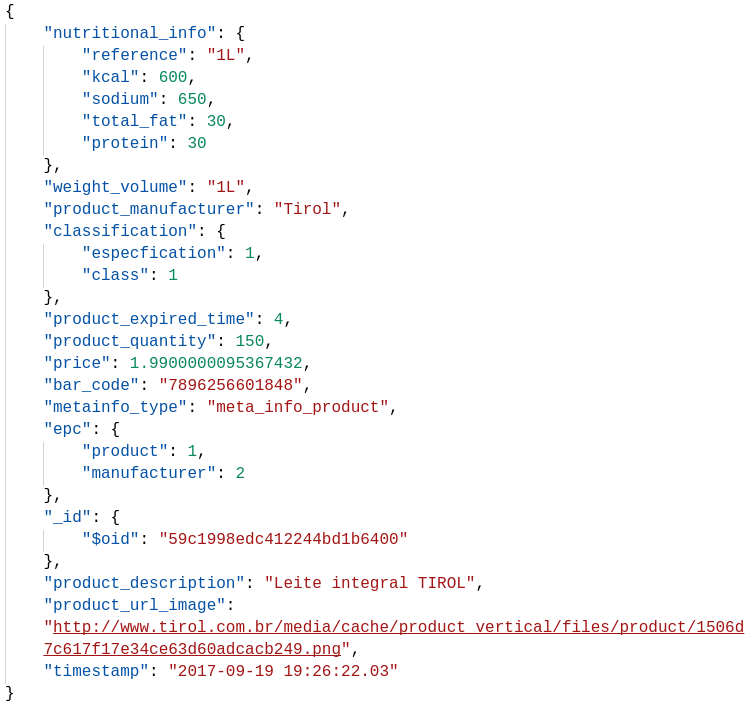
\includegraphics[width=0.9\textwidth]{cap4_metainfo}}
    
    \footnotesize{Fonte: Elaborado pelo Autor}
\end{quadro}

A primeira parte do registro indica as informações nutricionais, que poderão ser utilizadas, futuramente, na recomendação de produtos segundo uma dieta específica do usuário. A seguir, tem-se informações de peso/volume e fabricante.

Cada produto cadastrado é classificado em dois níveis: classe e especificação. O primeiro relaciona-se a um determinado tipo de produto como, por exemplo, bebidas e laticínios. A especificação determina qual produto em si é representado como, refrigerante e leite. Assim, torna-se possível recomendar produtos através da abordagem baseada em conteúdo.
Na sequência, é informado o tempo estimado em dias para considerar o produto adequado para consumo e, em seguida, a quantidade disponível no mercado, o preço unitário, o código de barras e o parâmetro que indica que o registro se trata da metainformação de um produto.

Outra informação relevante se refere aos parâmetros do código EPC que exemplares do produto terão. Considerando, novamente, o Quadro \ref{fig:cap4_epc}, tais parâmetros se referem ao fabricante e ao produto.

Por fim, tem-se informações de descrição do produto, de endereço da respectiva imagem ilustrativa e do instante em qual esse registro foi atualizado. Tanto a descrição como o endereço da imagem são empregados pela interface de usuário na demonstração do produto. 
%Já o instante do registro é utilizado pelo processo de sincronização de metainformação na verificação da necessidade por atualização do registro de metainformação.
Já o processo de sincronização de metainformação faz uso do momento do registro para verificar a necessidade por atualizações de metainformações.

% Metainfo de receitas
As receitas disponibilizadas possuem a estrutura demonstrada na Quadro \ref{fig:c4_recipe-meta}.
\begin{quadro}[htb]
    \caption{Registro de receita}
    \label{fig:c4_recipe-meta}
    \frame{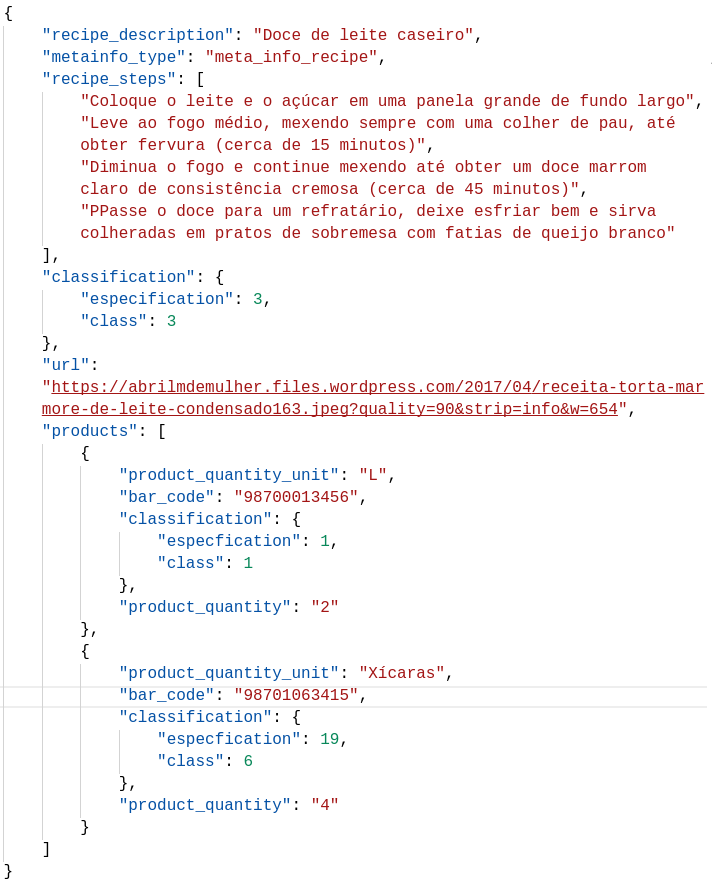
\includegraphics[width=0.8\textwidth]{c4_recipe-meta}}
    
    \footnotesize{Fonte: Elaborado pelo Autor}
\end{quadro}
Assim, a receita terá um nome ou uma descrição breve de seu conteúdo, além de um conjunto de passos para o preparo. Haverá também uma lista de produtos que fazem parte da receita, bem como suas respectivas classificações e quantidades necessárias à receita. Por fim, cada receita terá sua própria classificação, indicando que se trata de uma torta ou doce de leite, por exemplo. Tal informação de classificação é utilizada na recomendação de novas receitas.

%-----------------------------------------------------------%
\ProximoForaDoSumario 
\subsubsection{Base de Recomendações}

% TIPOS DE RECOMENDAÇÕES

Nessa base se encontram todos os diversos tipos de recomendação que o sistema pode prover, sendo elas: de compra de produtos faltantes, de novos produtos além de receitas selecionadas a partir do conteúdo da geladeira ou do perfil do usuário.

% Recomendação de produto
Cada recomendação de produto, independente do seu tipo, apresenta a estrutura demonstrada no Quadro \ref{fig:cap4_rec-prod}.

\begin{quadro}[htb]
    \caption{Registro de recomendação de produtos}
    \label{fig:cap4_rec-prod}
    \frame{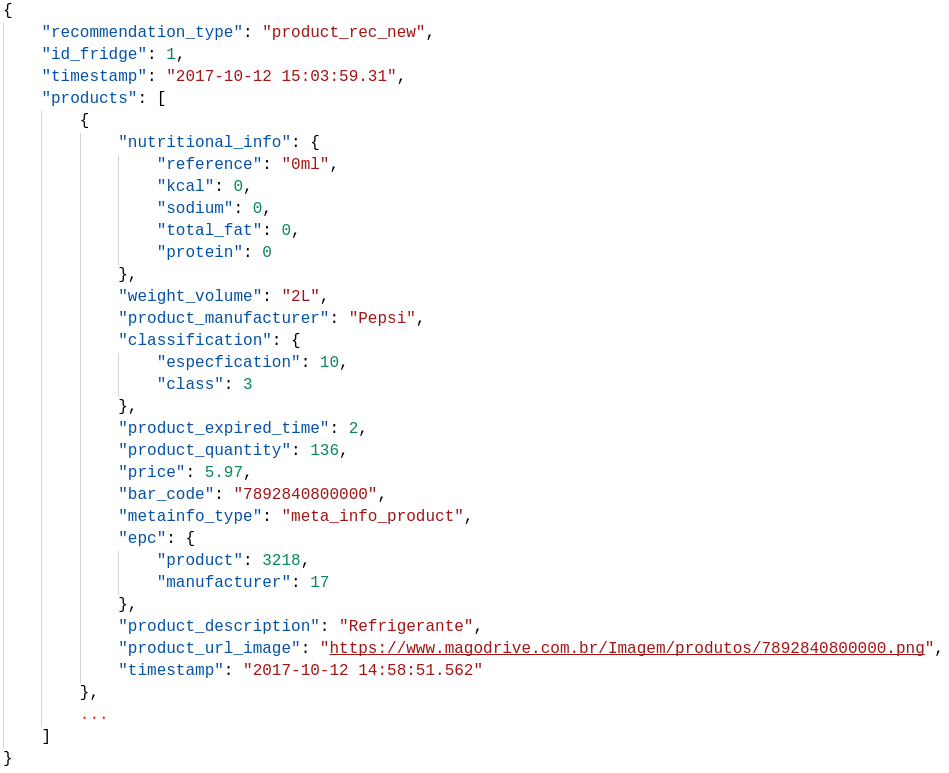
\includegraphics[width=\textwidth]{cap4_rec-prod}}
    
    \footnotesize{Fonte: Elaborado pelo Autor}
\end{quadro}

%%%%%%% aqui
No registro que consta no Quadro \ref{fig:cap4_rec-prod} é apresentada uma recomendação de um novo produto ao usuário. 
%Cada registro deste especifica a que tipo de registro se refere, ou seja, de produto faltante ou novo. 
Cada registro especifica o seu tipo, ou seja, uma recomendação de um produto faltante ou um novo.
Além disso, o momento em que a recomendação foi gerada é armazenado para diferenciar recomendações novas e antigas. A informação que segue no registro é a lista de produtos recomendados. Cada produto recomendado tem todo a sua metainformação anexada à recomendação.

% Recomendação de receita

O registro de recomendação de receitas, conforme Quadro \ref{fig:cap4_rec-recipe}, apresenta  as seguintes informações: o tipo de recomendação, além da identificação da geladeira à qual se refere, bem como o momento em que foi gerada. Por fim, um lista de receitas é apresentada, cada qual com a estrutura demonstrada na Seção \ref{sssec:metainfo}.

\begin{quadro}[htb]
    \caption{Registro de recomendação de receitas}
    \label{fig:cap4_rec-recipe}
    \frame{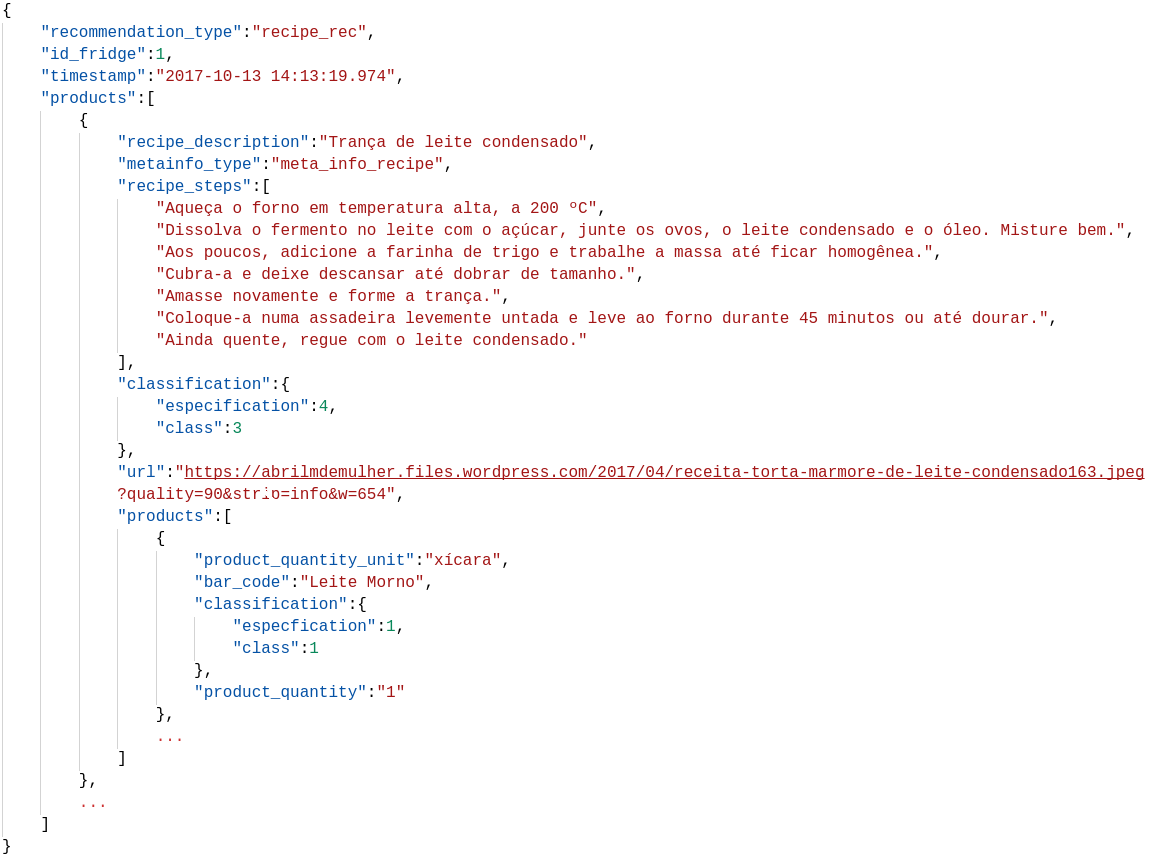
\includegraphics[width=\textwidth]{cap4_rec-recipe}}
    
    \footnotesize{Fonte: Elaborado pelo Autor}
\end{quadro}

%%%%%%%%%%%%%%%%%%%%%%%%%%%%%%%%%%%%%%%%%%%%%%%%%%%%%%%%

\subsection{Camada de Processamento}

Nas próximas seções, os aspectos da implementação dos processos serão detalhados.
%%%%%%%%%%%%%%%%%%%%%%%%%%%%%%%%%%%%%%%%%%%%%%%%%%%%%%%%%%%%%%%%%%%%%%%%%%%

\ProximoForaDoSumario 
\subsubsection{Processo de Compras Automáticas}

A compra automática ocorre quando existirem listas de compras pendentes na base de estruturas auxiliares. Quando isso ocorrer o processo deve contatar o serviço de compras do mercado para efetuar a aquisição definida pelo usuário. Isso é realizado a partir de uma requisição HTTP que é enviada ao serviço do mercado contendo a lista de produtos requeridos e as respectivas quantidades.

%%%%%%%%%%%%%%%%%%%%%%%%%%%%%%%%%%%%%%%%%%%%%%%%%%%%%%%%%%%%%%%%%%%%%%%%%%%
\ProximoForaDoSumario 
\subsubsection{Processo de Geração de Recomendações} \label{sssec:proc_ger_rec}

Neste trabalho, implementou-se quatro formas distintas de recomendação conforme descrito a seguir, sendo elas, recomendação de produtos faltantes ou novos, além de receitas a partir do conteúdo disponível ou do perfil.

\begin{itemize}
    \item \textbf{Recomendação de Produtos Faltantes}
\end{itemize}

A recomendação de produtos faltantes baseia-se na ideia de lembrar ao usuário quando determinados produtos considerando essenciais estão em falta e efetuar a compra desses itens. Assim, o usuário será alertado quando isso ocorrer e poderá decidir se aceita que se efetive a compra ou não.

Para que as recomendações sejam possíveis são necessárias duas informações: lista de produtos essenciais, obtida a partir das configurações de usuário, e da lista de interações. 

A partir dessas informações, um processo em segundo plano, periodicamente, verificará a necessidade da compra desses produtos.

Para a geração das recomendações, inicialmente será criada uma lista com os produtos contidos atualmente na geladeira e suas respectivas quantidades, a partir do conjunto de registros de interações. Em seguida, será comparado produtos requisitados com as respectivas quantidades de produtos existentes e, então, uma lista com os itens em falta será criada e gravada na base de registros de recomendação.
 
% Inicialmente, será criada uma lista de produtos contidos atualmente   e suas respectivas quantidades, a partir do conjunto de registros de interações. Em seguida, será comparado produtos requisitados com as respectivas quantidades de produtos existentes e, então, uma lista com os itens em falta será criada e gravada na base de registros de recomendação.

\begin{itemize}
    \item \textbf{Recomendação de Produtos Novos}
\end{itemize}

A recomendação de produtos novos tem como princípio fundamental o conceito de filtragem colaborativa, descrita na Seção \ref{sec:filtragem-colaborativa}. Assim, sugestões são criadas a partir da comparação entre usuários com preferências parecidas. Tendo conhecimento do usuário com maior semelhança, é possível recomendar produtos que um usuário interagiu mas que o outro não conhece. Apesar de não conhecer o produto sugerido, a probabilidade de a recomendação agradar o usuário é alta, já que a sugestão emergiu de um usuário com perfil similar.

A comparação entre usuários foi realizada utilizando da correlação de Pearson, descrita na Seção \ref{sssec:similaridade}. As informações utilizadas para as sugestões de itens são compostas pelos registros de interações e as metainformações dos produtos. 

Primeiramente, uma matriz idêntica à matriz da Tabela \ref{tab:matriz-av-item-user} foi construída. No entanto, cada par de usuário e item é interpretado como o número de interações entre usuário e item, ao contrário da matriz de avaliação da tabela mencionada. A partir da matriz, é possível calcular a média de interações para cada usuário. Tendo o número de interações entre cada usuário e cada item além da média de interações, é possível obter a similaridade entre cada usuário.

A partir da similaridade entre usuários, ordena-se uma lista de usuários de maneira descendente, tendo como referência o usuário ao qual deseja-se recomendar um item.
Após isso, a lista ordenada é percorrida. Para cada usuário presente nela, é calculada uma subtração de conjuntos envolvendo tal indivíduo e o usuário de receberá as recomendações. Tais conjuntos se referem aos produtos aos quais cada usuário interagiu. E, como consequência do cálculo, o conjunto de itens resultantes releva os produtos aos quais o usuário de referência ainda não interagiu mas o outro o fez. Por fim, o resultado é adicionado ao conjunto de recomendação.

%
%A seguir, começando pelo primeiro usuário da lista de semelhantes, se faz a subtração de conjunto de produtos interagidos por este em relação ao usuário de referência. Desse modo, tem-se um conjunto de produtos que o usuário ainda não interagiu. 
%
Assim, o processo será realizado para os demais usuários da lista até que se atinja um conjunto de produtos com a quantidade desejada que, então, será registrado na base de recomendações.

\begin{itemize}
    \item \textbf{Recomendação de Receitas com Base nos Produtos Disponíveis}
\end{itemize}

Este tipo de recomendação objetiva selecionar as receitas que englobem em seu conteúdo apenas os itens disponíveis, tanto quanto possível. Para o cálculo das recomendações, são necessárias as metainformações dos produtos e receitas, além dos registros de interação. Assim, é possível comparar produtos atuais com os itens contidos em receitas.

Cada receita não especifica um produto em particular, mas deixa claro a classificação do produto. Assim, ao invés de especificar uma caixa de leite da marca X, deixa restrito a um produto que é um laticínio e, mais especificamente, uma caixa de leite.

Para o processo de criação de recomendação, inicialmente, a lista de itens atualmente contidos na geladeira é criada. Após isso, para cada receita na base de dados é contabilizado o número de itens presentes na receita e na geladeira. Em seguida, ordena-se a lista de receitas começando por aquela que contém o maior número de correspondências entre receita e conteúdo. Por fim, um conjunto contendo as primeiras receitas da lista é gravado na base como uma recomendação já efetuada.

\begin{itemize} 
    \item \textbf{Recomendação de Receitas com Base no Perfil do Usuário}
\end{itemize}

As recomendações de receitas a partir do perfil do usuário buscam trazer receitas ao usuário a partir das suas preferências por produtos em específico. Assim, seleciona-se receitas que contenham produtos que o usuário tem maior preferência. As informações necessárias à recomendação são as interações dos usuários e as metainformações de produtos e receitas.

Para gerar as sugestões, inicialmente cria-se uma lista com todos os produtos com os quais o usuário em questão interagiu e as contagens de interações com cada produto. Seleciona-se, em seguida, o conjunto de produtos com maior frequência de interações. Por fim, seleciona-se receitas que contenham tais produtos%, da mesma forma que a recomendação por conteúdo disponível.

%%%%%%%%%%%%%%%%%%%%%%%%%%%%%%%%%%%%%%%%%%%%%%%%%%%%%%%%%%%%%%%%%%%%%%%%%%%
\ProximoForaDoSumario 
\subsubsection{Processo de Sincronização de metainformação}

A sincronização é feita a partir da comparação entre os momentos em que se criou o registro presente na base de metainformação e o registro contido no mercado. Caso o registro do mercado seja mais recente, esse será enviado para o servidor para atualização do registro. 

Para que a sincronização seja possível, em cada metainformação tem-se um campo chamado  \textit{timestamp} que indica a data de criação de tal registro. Por fim, a operação de sincronização deve ser realizada periodicamente por um processo em segundo plano. 
%A implementação desse processo não foi executada devido a falta de tempo e o fato de não ser essencial ao trabalho.


%%%%%%%%%%%%%%%%%%%%%%%%%%%%%%%%%%%%%%%%%%%%%%%%%%%%%%%%
\subsection{Camada de Agente Externo}

A camada descrita nesta seção refere-se ao componente independente do modelo proposto, isto é, o mercado. Ele possui um sistema próprio, mas que disponibiliza um conjunto de serviços pelos quais é possível a interação externa. O primeiro serviço é a sincronização de metainformação de produtos, onde periodicamente serão verificadas alterações, ou inserções de novos produtos. Caso existam dados desatualizados, estes serão enviados ao servidor principal.

Além disso, há o serviço de compras, onde uma lista de produtos será informada em conjunto com as respectivas quantidades. Uma verificação de disponibilidade dos itens solicitados será realizada e, como retorno, o serviço indica quais produtos foram adquiridos com sucesso e quais não puderam ser atendidos. Vale destacar que, apesar de a verificação de disponibilidade ser realizada antes mesmo da sugestão ao usuário, é possível que o produto acabe até o momento em que a compra seja realmente solicitada.
